% Provenance (never printed): see sources/outline_sources.md (Year 3: the
% structure of the Galaxy; the rotation curve and dark matter; galaxy types;
% the distance ladder, Hubble's law recalled from the physics books).
% Brief: sources/book5/BRIEFS.md, ch. 29. Curves from figdata/bachelor-3/
% rotation_curve.py (the circular velocity curve of Eilers et al. 2019 with the
% Pouliasis et al. 2017 Model I baryons and an NFW halo fitted to it) and
% distance_ladder.py (the OGLE-IV Cepheids of the Large Magellanic Cloud, CDS
% J/AcA/65/297, and the ranges of the rungs). Exercise and problem values in the
% Book 5 scratch calculator calc/ch29.py. The survey of Part I of the problem and
% the galaxies of the exercises are invented.
\chapter{आकाशगंगा और मंदाकिनियाँ}\label{ch:b3:milky-way-galaxies}

सौरमंडल में सूर्य से दूर के ग्रह धीरे चलते हैं: बुध उसकी परिक्रमा
\qty{47.4}{km.s^{-1}} की चाल से करता है, नेप्च्यून \qty{5.4}{km.s^{-1}} की चाल से, जैसा
केपलर का तीसरा नियम एक केंद्रीय द्रव्यमान से बँधे पिंडों से यही माँगता है। आकाशगंगा के तारे
ऐसा व्यवहार नहीं करते। बीस हज़ार से अधिक लाल दानवों की गतियों से मापने पर
उनकी वृत्तीय कक्षाओं की चाल
केंद्र से \qty{5}{kpc} पर \qty{227}{km.s^{-1}}, सूर्य पर \qty{229}{km.s^{-1}},
और \qty{25}{kpc} पर, जहाँ शायद ही कोई तारे या गैस
बचे हों, अब भी \qty{198}{km.s^{-1}} है। यदि दिखने वाला द्रव्यमान ही सब कुछ होता, तो बाहरी
तारे कहीं अधिक धीमे होते। कुछ अदृश्य चीज़ उन्हें थामे रखती है। यह अध्याय
हमारी आकाशगंगा का वर्णन करता है, उसके घूर्णन से उसका भार ज्ञात करता है,
अन्य मंदाकिनियों को प्रकारों में छाँटता है, और उन विधियों की श्रृंखला पर चढ़ता है
जिनसे उनकी दूरियाँ और ब्रह्मांड का विस्तार मापे जाते हैं।
% ledger: planet:Mercury.vorb, planet:Neptune.vorb, eilers19:vc, eilers19:table1

\begin{recall}
आकाशगंगा, डॉप्लर प्रभाव, केपलर के नियम, गोलीय कोश के आकर्षण पर न्यूटन का प्रमेय,
अदीप्त द्रव्य, कृष्ण विवर और उनकी श्वार्ज़्शील्ड त्रिज्या, अधिनवतारा,
श्वेत वामन, परमाणु हाइड्रोजन की 21-cm रेखा और हबल का नियम भौतिकी की पुस्तकों में हैं।
वार्षिक लंबन, पारसेक, फ़्लक्स और दीप्ति, दृश्य और निरपेक्ष कांतियाँ,
दूरी-मापांक, प्रकाशमितीय बैंड और वर्ण-सूचकांक
पुस्तक 3 (स्नातक वर्ष 1) में हैं, उसके दूरबीनों और प्रकाशमिति वाले अध्याय में।
अंतरतारकीय माध्यम और उसकी धूल
पुस्तक 4 (स्नातक वर्ष 2) में हैं, उसके
अंतरतारकीय माध्यम और तारा निर्माण वाले अध्याय में।
\end{recall}

\section{आकाशगंगा की संरचना}\label{sec:b3:milky-way-galaxies:structure}

पृथ्वी से देखने पर आकाशगंगा पूरे आकाश में फैली प्रकाश की एक पट्टी के रूप में दिखती है,
जिसे धूल की काली धारियाँ पार करती हैं और जो नक्षत्र धनु की ओर सबसे चमकीली है,
जहाँ उसका केंद्र स्थित है। यह पट्टी वह चक्रिका है जिसमें सूर्य स्थित है,
जिसे भीतर से किनारे की ओर से देखा गया है।

\begin{omfigure}
\centering
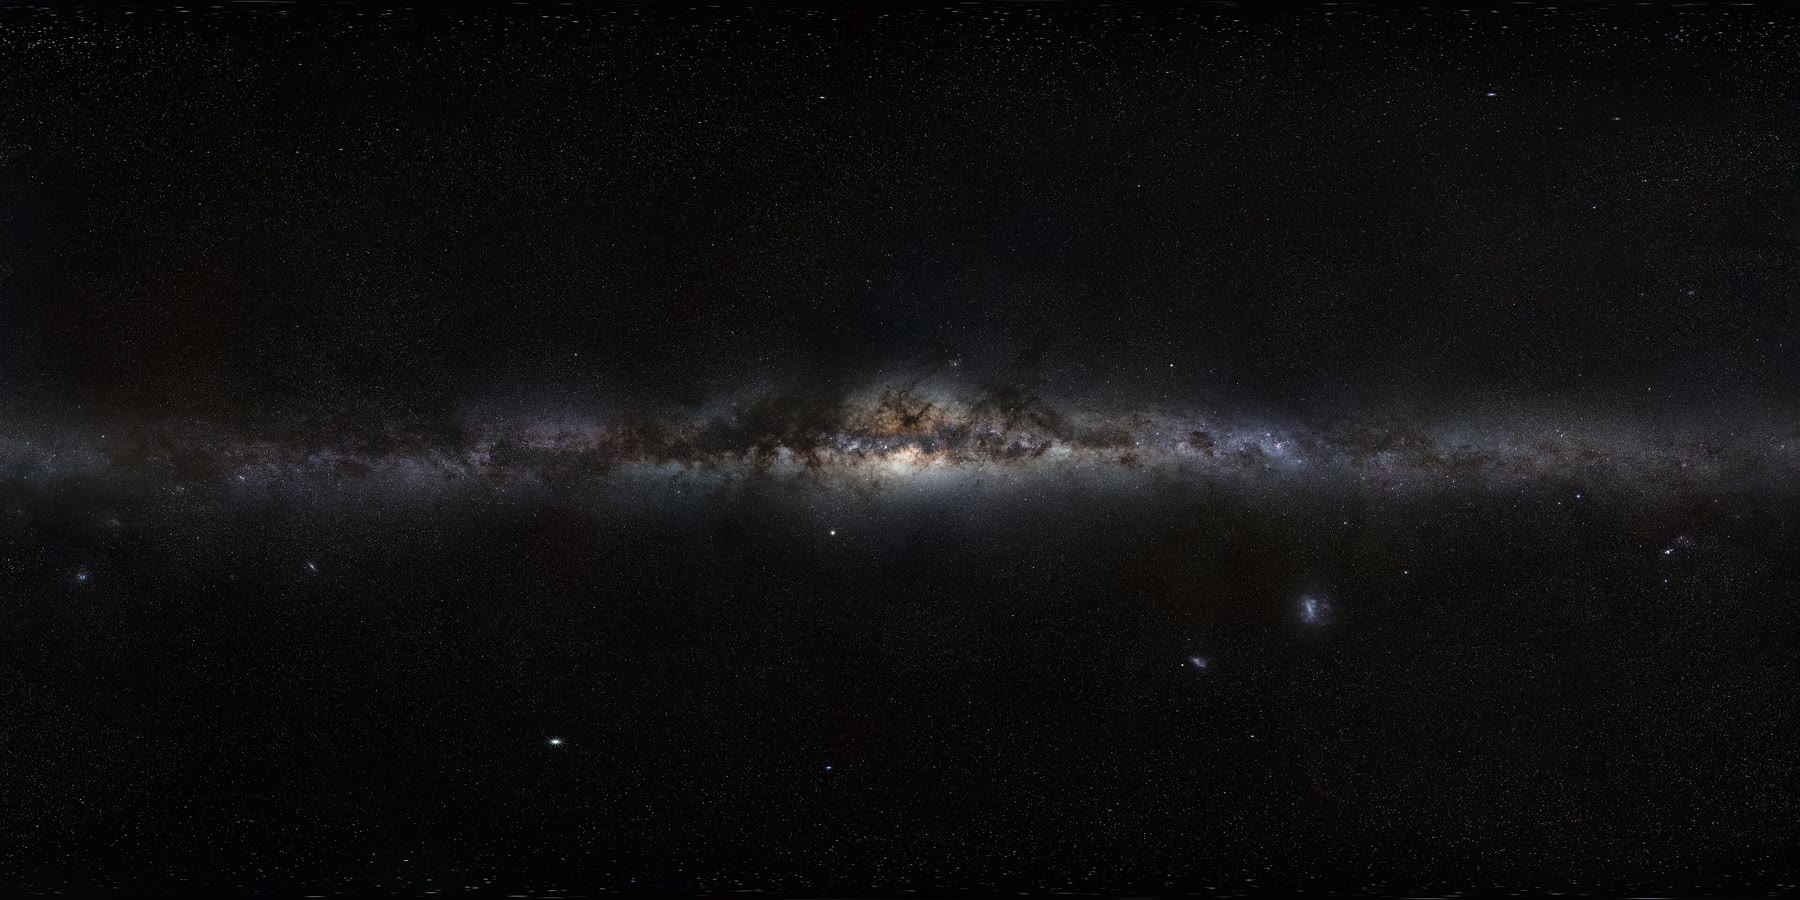
\includegraphics[width=0.96\linewidth]{images/book5/b3-milky-way-panorama.jpg}
\par\smallskip{\small पूरा आकाश एक ही चित्र में, इस प्रकार प्रक्षेपित कि आकाशगंगा का तल
बीच में आड़ा जाए और उसका केंद्र
चित्र के केंद्र पर हो। पट्टी भीतर से देखी गई चक्रिका है; काली
धारियाँ चक्रिका की धूल हैं जो उनके पीछे के तारों को छिपाती है; केंद्रीय उभार
केंद्र के चारों ओर फूला है। पट्टी के नीचे, दाईं ओर, दो छोटे धब्बे
बृहत् और लघु मैगेलैनिक मेघ हैं, दो उपग्रह मंदाकिनियाँ;
पट्टी के नीचे बाईं किनारे के पास का धुंधला धब्बा एंड्रोमेडा
मंदाकिनी है। फ़ोटो ESO/S.~Brunier, CC BY~4.0।}\label{fig:b3:milky-way-galaxies:panorama}
\end{omfigure}
% ledger: photo:b3-milky-way-panorama, mcconn12:local-group

\begin{definition}[मंदाकिनीय चक्रिका, मोटी चक्रिका, मंदाकिनीय उभार और तारकीय प्रभामंडल]\label{def:b3:milky-way-galaxies:structure}
\emph{मंदाकिनीय चक्रिका}\index{मंदाकिनीय चक्रिका} आकाशगंगा का चपटा घटक है,
जो तारों, गैस और धूल से बना है और अपने केंद्र के चारों ओर लगभग वृत्तीय कक्षाओं में घूमता है;
इसका घनत्व अपने मध्य-तल से ऊँचाई के साथ और केंद्र से दूरी के साथ लगभग चरघातांकी
रूप से घटता है, एक ऊँचाई-मापक और एक लंबाई-मापक के पैमाने पर।
\emph{मोटी चक्रिका}\index{मोटी चक्रिका} एक दूसरी, अधिक पुरानी
चक्रिका है, जिसका ऊँचाई-मापक बड़ा और द्रव्यमान छोटा है। मंदाकिनीय उभार
\emph{मंदाकिनीय उभार}\index{मंदाकिनीय उभार} तारों का वह केंद्रीय जमाव है जो
चक्रिका से बाहर की ओर फूला होता है। \emph{तारकीय प्रभामंडल}\index{तारकीय प्रभामंडल} वह
विरल, लगभग गोलाभ घटक है जो पुराने तारों और
गोलीय गुच्छों से बना है, और चक्रिका तथा उभार को घेरता है।
\end{definition}

आकाशगंगा एक पट्टीदार सर्पिल है। सूर्य के आसपास पतली
चक्रिका का ऊँचाई-मापक लगभग \qty{300}{pc} है और \omterm{def:b3:milky-way-galaxies:structure}{मोटी चक्रिका} का
लगभग \qty{900}{pc}; उनके लंबाई-मापक लगभग \qty{2.6}{kpc} और
\qty{2.0}{kpc} हैं। \omterm{def:b3:milky-way-galaxies:structure}{मोटी चक्रिका} में लगभग \num{6e9} सौर द्रव्यमान हैं,
पतली चक्रिका का लगभग पाँचवाँ भाग। किनारे से देखने पर उभार एक बक्से
या मूँगफली जैसा होता है: यह तारों की एक पट्टी का मोटा हुआ भीतरी भाग है, लगभग
\qty{5}{kpc} अर्ध-लंबाई की, जिसकी लंबी अक्ष सूर्य से केंद्र की ओर जाने वाली रेखा से
\ang{27} का कोण बनाती है। \omterm{def:b3:milky-way-galaxies:structure}{तारकीय प्रभामंडल} में
तारों का लगभग केवल एक प्रतिशत है। कुल मिलाकर आकाशगंगा के तारों का
भार लगभग \num{5e10} सौर द्रव्यमान है।
% ledger: bhg16:structure

\begin{omfigure}
\centering
\begin{tikzpicture}[x=0.17cm, y=0.17cm, font=\scriptsize]
% edge-on view
\begin{scope}
\fill[omProp!8] (0,0) circle (17);
\draw[omProp!60, densely dotted] (0,0) circle (17);
\fill[black!12] (0,0) ellipse (15 and 2.4);
\fill[black!30] (0,0) ellipse (15 and 0.8);
\fill[black!45] (-3.2,0) .. controls (-3.4,2.3) and (-1.2,2.0) .. (0,1.4)
  .. controls (1.2,2.0) and (3.4,2.3) .. (3.2,0)
  .. controls (3.4,-2.3) and (1.2,-2.0) .. (0,-1.4)
  .. controls (-1.2,-2.0) and (-3.4,-2.3) .. (-3.2,0) -- cycle;
\foreach \p in {(-10,9),(6,12),(12,-7),(-6,-13),(-13,-4),(3,-9),(12,8)}
  \fill[omProp] \p circle (0.35);
\fill[ocYellow, draw=black] (-8.2,0.15) circle (0.55);
\node[anchor=south] at (-8.2,0.9) {सूर्य};
\draw[|<->|] (0,-4.6) -- node[below] {$R_0 \approx \qty{8.2}{kpc}$} (-8.2,-4.6);
\node[anchor=west] at (15.3,0) {पतली चक्रिका};
\node[anchor=west] at (13.2,2.8) {मोटी चक्रिका};
\draw[->] (4.6,4.6) node[anchor=south west, inner sep=1pt] {उभार} -- (2.4,1.7);
\node[omProp!80!black] at (-11,13.5) {तारकीय प्रभामंडल};
\node at (0,-19.5) {(क) किनारे से देखा गया};
\end{scope}
% face-on view
\begin{scope}[xshift=7.6cm]
\fill[omProp!8] (0,0) circle (17);
\draw[omProp!60, densely dotted] (0,0) circle (17);
\fill[black!12] (0,0) circle (15);
\foreach \a in {0,180} {
  \draw[line width=1.6pt, black!40, rotate=\a+63]
    plot[domain=0:3.9, samples=50] ({5*exp(0.25*\x)*cos(\x r)}, {5*exp(0.25*\x)*sin(\x r)});
}
\fill[black!45, rotate=63] (0,0) ellipse (5 and 1.5);
\draw[dashed] (0,0) circle (8.2);
\fill[ocYellow, draw=black] (0,-8.2) circle (0.55);
\node[anchor=north] at (0,-8.9) {सूर्य};
\draw[dotted, thick] (0,0) -- (0,-8.2);
\draw[thick, ->] (0,0) ++(25:16) arc (25:-25:16);
\node[anchor=west] at (17.3,0) {घूर्णन};
\node[anchor=west, fill=black!12, inner sep=1pt] at (3.4,3.4) {पट्टी};
\draw[|-|] (6,-15.5) -- node[below] {\qty{5}{kpc}} (11,-15.5);
\node at (0,-19.5) {(ख) उत्तरी मंदाकिनीय ध्रुव से देखा गया};
\end{scope}
\end{tikzpicture}
\par\smallskip{\small आकाशगंगा का रेखाचित्र, इसके मुख्य आयामों के लिए मापानुसार
आरेखित। (क)~किनारे से देखा गया: पतली चक्रिका (गहरी पट्टी), \omterm{def:b3:milky-way-galaxies:structure}{मोटी चक्रिका} (हल्की
पट्टी), चपटा उभार, और गोलीय गुच्छों (नारंगी बिंदु) सहित \omterm{def:b3:milky-way-galaxies:structure}{तारकीय प्रभामंडल}; सूर्य चक्रिका में
स्थित है, केंद्र से लगभग \qty{8.2}{kpc} दूर
और मध्य-तल से लगभग \qty{25}{pc} ऊपर (इतना छोटा कि दिखाया न जा सके)।
(ख)~उत्तरी मंदाकिनीय ध्रुव से देखने पर: पट्टी, लगभग
\qty{5}{kpc} अर्ध-लंबाई की, सूर्य से केंद्र की ओर की रेखा से \ang{27} झुकी हुई
(बिंदीदार); सौर वृत्त (डैश वाला); सर्पिल भुजाएँ योजनाबद्ध रूप से खींची गईं;
इस दृश्य में आकाशगंगा दक्षिणावर्त घूमती है।}\label{fig:b3:milky-way-galaxies:sketch}
\end{omfigure}
% ledger: bhg16:structure, gravity19:r0

\begin{definition}[तारकीय समष्टि]\label{def:b3:milky-way-galaxies:populations}
एक \emph{तारकीय समष्टि}\index{तारकीय समष्टि} किसी मंदाकिनी के तारों का एक समूह है
जिसके तारे आयु, रासायनिक संघटन और कक्षाओं की एक परास साझा करते हैं।
पतली चक्रिका के युवा तारे, जो हीलियम से भारी तत्त्वों से समृद्ध हैं
और लगभग वृत्ताकार कक्षाओं में हैं, परंपरागत रूप से समष्टि~I कहलाते हैं;
प्रभामंडल और गोलीय गुच्छों के पुराने तारे, जो
भारी तत्त्वों में निर्धन हैं और जिनकी कक्षाओं में बड़ी यादृच्छिक गतियाँ हैं तथा शुद्ध घूर्णन कम है,
समष्टि~II कहलाते हैं।
\end{definition}

\omterm{def:b3:milky-way-galaxies:structure}{मोटी चक्रिका} इन दोनों के बीच स्थित है: इसके तारे अधिकतर
पतली चक्रिका के तारों से पुराने हैं और, दिए गए लोह-अंश पर, हल्के तत्त्वों में समृद्ध हैं,
जिन्हें खगोलविद अल्फ़ा तत्त्व कहते हैं, जिनका मापन लोहे के सापेक्ष किया जाता है।
\omterm{def:b3:milky-way-galaxies:structure}{तारकीय प्रभामंडल} एक
जीवाश्म अभिलेख है: इसका अधिकांश भाग छोटी मंदाकिनियों से बना है जो
आकाशगंगा में गिरीं और इसके ज्वार से टूट गईं, और उनकी कुछ तारा-धाराएँ
आज भी आकाश में अनुसरित की जा सकती हैं।
% ledger: bhg16:populations

\begin{definition}[मंदाकिनीय निर्देशांक]\label{def:b3:milky-way-galaxies:coordinates}
किसी दिशा के \emph{मंदाकिनीय निर्देशांक}\index{मंदाकिनीय निर्देशांक} ये हैं:
उसका \emph{मंदाकिनीय अक्षांश} $b$, जो मंदाकिनीय तल से कोण है
(उत्तरी मंदाकिनीय ध्रुव की ओर धनात्मक), और उसका \emph{मंदाकिनीय
देशांतर} $\ell$, जो तल में मंदाकिनीय केंद्र की दिशा ($\ell = 0$) से
$\ell = \ang{90}$ तक मापा जाता है, वह दिशा जिधर
आकाशगंगा का घूर्णन सूर्य को ले जाता है। यह तल
1958 में आकाशगंगा के प्रमुख परमाणु हाइड्रोजन तल के रूप में परिभाषित किया गया था;
उत्तरी मंदाकिनीय ध्रुव का दक्षिणावर्त आरोहण \ang{192.25}
($12^\mathrm{h}49^\mathrm{m}$) और क्रांति \ang{27.4} पर स्थित है
(विषुव 1950)।
\end{definition}
% ledger: liu11:galactic, reid20:sgra

सूर्य तल में पूरी तरह नहीं है: वह उससे लगभग \qty{25}{pc} उत्तर में है।
केंद्र से उसकी दूरी, $R_0$, लंबे समय तक मंदाकिनीय खगोल-विज्ञान की
सबसे अनिश्चित संख्या रही। अब इसे ज्यामितीय रूप से मापा जाता है: तारा S2
आकाशगंगा के केंद्रीय कृष्ण विवर का चक्कर \num{16}-वर्षीय कक्षा में लगाता है।
आकाश में कोणीय आकार तथा दृष्टि-रेखा के अनुदिश वेग,
27 वर्षों तक अनुसरित करने पर, केंद्र तक की दूरी सीधे देते हैं:
$R_0 = \qty{8178}{pc}$, जिसकी सांख्यिकीय त्रुटि \qty{13}{pc} और व्यवस्थित
त्रुटि \qty{22}{pc} है। सभी विधियों की समीक्षा
$R_0 = \qty[separate-uncertainty=true]{8.2 \pm 0.1}{kpc}$ देती है।
% ledger: bhg16:structure, gravity19:r0

\section{घूर्णन और अदीप्त-द्रव्य प्रभामंडल}\label{sec:b3:milky-way-galaxies:rotation}

\begin{definition}[स्थानीय विराम मानक]\label{def:b3:milky-way-galaxies:lsr}
\emph{स्थानीय विराम मानक}\index{स्थानीय विराम मानक} (LSR) वह संदर्भ-तंत्र है
जो मंदाकिनीय केंद्र के परितः उस वृत्ताकार कक्षा पर चलता है
जो सूर्य की वर्तमान स्थिति से होकर गुजरती है। निकटवर्ती तारों और गैस के वेग
इसके सापेक्ष दिए जाते हैं।
\end{definition}

सूर्य LSR के सापेक्ष लगभग \qty{10}{km.s^{-1}} की गति से मंदाकिनीय केंद्र की ओर,
\qty{11}{km.s^{-1}} घूर्णन की दिशा में और
\qty{7}{km.s^{-1}} उत्तरी मंदाकिनीय ध्रुव की ओर गति करता है: एक छोटी विशिष्ट गति,
जो कुछ सौ किलोमीटर प्रति सेकंड की गति $V_0$ वाली कक्षा के ऊपर होती है।
पृथ्वी से देखने पर आकाशगंगा के केंद्र का रेडियो स्रोत
मंदाकिनीय तल के अनुदिश प्रति वर्ष \qty{6.411}{mas} बहता दिखता है;
इस बहाव का लगभग सब कुछ सूर्य की कक्षा का प्रतिबिंब है, और इससे सूर्य की
केंद्र के परितः कुल गति, \qty[separate-uncertainty=true]{248 \pm 3}{km.s^{-1}}
प्राप्त होती है (\cref{exo:b3:milky-way-galaxies:2} देखिए)।
% ledger: bhg16:lsr, reid20:sgra

\begin{definition}[घूर्णन वक्र; ऊर्ट स्थिरांक]\label{def:b3:milky-way-galaxies:rotation-curve}
किसी चपटी मंदाकिनी की \emph{घूर्णन वक्र}\index{घूर्णन वक्र} उसके तल में
वृत्ताकार कक्षा की गति $V(R)$ है, जो
उसके केंद्र से दूरी $R$ का फलन है। आकाशगंगा के लिए, $V_0 = V(R_0)$ और
$V'_0 = \mathrm{d}V/\mathrm{d}R$ को $R_0$ पर लेकर, \emph{ऊर्ट
स्थिरांक}\index{ऊर्ट स्थिरांक} होते हैं
\[
A = \frac12\left(\frac{V_0}{R_0} - V'_0\right), \qquad
B = -\frac12\left(\frac{V_0}{R_0} + V'_0\right).
\]
\end{definition}

$A$ चकती के घूर्णन के अपरूपण को और $B$ उसकी भ्रमिलता को मापता है: ठोस पिंड की भाँति घूमती
चकती में $V'_0 = V_0/R_0$ और $A = 0$ होता है; सपाट \omterm{def:b3:milky-way-galaxies:rotation-curve}{घूर्णन वक्र} पर
$A = -B$ होता है। उनका अंतर LSR का कोणीय वेग है,
$A - B = V_0/R_0 = \omega_0$, और उनका योग ढाल है, $A + B = -V'_0$।

\begin{theorem}[ऊर्ट के सूत्र]\label{thm:b3:milky-way-galaxies:oort}
सूर्य से $d \ll R_0$ दूरी पर, मंदाकिनीय तल में
देशांतर $\ell$ पर स्थित, वृत्ताकार कक्षा में चलने वाला एक तारा LSR के सापेक्ष
अरीय वेग $v_r$ और अनुप्रस्थ वेग $v_t$ ($\ell$ बढ़ने की
दिशा में धनात्मक) रखता है
\[
v_r = A\,d\sin 2\ell, \qquad v_t = d\,(A\cos 2\ell + B),
\]
$d/R_0$ में प्रथम कोटि तक।
\end{theorem}

\begin{proof}
मान लीजिए $\omega(R) = V(R)/R$ कक्षा का, $R$ पर, कोणीय वेग है।
मंदाकिनीय केंद्र को मूलबिंदु पर रखिए, सूर्य को दूरी $R_0$ पर, और मान लीजिए तारा
केंद्र से दूरी $R$ पर है, और केंद्र से देखी गई उसकी स्थिति
सूर्य की स्थिति के साथ कोण $\theta$ बनाती है।
तारे के वेग $\omega R$ और LSR के वेग $\omega_0 R_0$ को दृष्टि-रेखा पर प्रक्षेपित करने पर,
सूर्य--तारा--केंद्र त्रिभुज में थोड़ी त्रिकोणमिति (ज्या-नियम
$R\sin(\ell + \theta) = R_0\sin\ell$ देता है) से सटीक परिणाम
$v_r = R_0\,[\omega(R) - \omega_0]\sin\ell$ प्राप्त होता है। इसी प्रकार,
दृष्टि-रेखा के लंबवत दिशा में,
$v_t = R_0\,[\omega(R) - \omega_0]\cos\ell - \omega(R)\,d$ प्राप्त होता है। निकटवर्ती तारे के लिए,
$\omega(R) - \omega_0 \approx \omega'_0\,(R - R_0)$ और
$R - R_0 \approx -d\cos\ell$ है। तब
$v_r \approx -R_0\omega'_0\,d\cos\ell\sin\ell = -\tfrac12 R_0\omega'_0\,
d\sin 2\ell$ और प्रथम-कोटि पदों को रखने पर,
$v_t \approx -R_0\omega'_0\,d\cos^2\ell - \omega_0 d$ प्राप्त होता है।
$\omega'_0 = V'_0/R_0 - V_0/R_0^2$ रखने पर, $-\tfrac12 R_0\omega'_0 = A$ और
$-R_0\omega'_0\cos^2\ell - \omega_0 = A(1 + \cos 2\ell) - (A - B) =
A\cos 2\ell + B$।
\end{proof}

निकटवर्ती तारों के दृष्टि-वेग इसलिए आकाश में घूमते हुए $\sin 2\ell$ के अनुसार बदलते हैं,
और उनकी स्वगतियाँ $\cos 2\ell$ के अनुसार, $B$ से निर्धारित माध्य के चारों ओर बदलती हैं।
गैया की पहली सूची के \num{304267} तारों की स्वगति और लंबन से,
लगभग \qty{230}{pc} की विशिष्ट दूरी पर, \omterm{def:b3:milky-way-galaxies:rotation-curve}{ऊर्ट स्थिरांक}
$A = \qty[separate-uncertainty=true]{15.3 \pm 0.4}{km.s^{-1}.kpc^{-1}}$
और $B = \qty[separate-uncertainty=true]{-11.9 \pm 0.4}{km.s^{-1}.kpc^{-1}}$ प्राप्त हुए।
अक्षसममित चक्रिका में न होने वाले दो और पद, जिन्हें $C$
और $K$ कहते हैं, लगभग \qty{-3}{km.s^{-1}.kpc^{-1}} आए: स्थानीय चक्रिका
पट्टी और सर्पिल भुजाओं से विक्षोभित है।
% ledger: bovy17:oort

\subsection*{21-सेंटीमीटर रेखा से घूर्णन वक्र}

परमाणु हाइड्रोजन चक्रिका को भरता है और 21-सेंटीमीटर रेखा उत्सर्जित करता है,
\qty{1420.405751}{MHz} पर; रेडियो तरंगें उस धूल के आर-पार जाती हैं जो
दृश्य तरंगदैर्घ्य पर दूर की चक्रिका को छिपाती है। तल में किसी दृष्टि-रेखा के
अनुदिश, गैस का हर बादल अपनी रेखा को अपने दृष्टि-वेग के
डॉप्लर विस्थापन पर जोड़ता है, और रेखा की प्रोफ़ाइल वेगों का
स्पेक्ट्रम होती है। सौर वृत्त के भीतर एक वेग विशेष रूप से चुना जाता है।
% ledger: nrao:hi-line

\begin{theorem}[स्पर्शबिंदु विधि]\label{thm:b3:milky-way-galaxies:tangent}
मान लीजिए गैस वृत्तीय कक्षाओं में घूमती है, जिनका कोणीय वेग $\omega(R)$ है
और जो बाहर की ओर घटता है। देशांतर
$0 < \ell < \ang{90}$ की किसी दृष्टि-रेखा के अनुदिश, LSR के सापेक्ष दृष्टि-वेग
स्पर्शबिंदु पर सबसे बड़ा होता है, जहाँ दृष्टि-रेखा किसी कक्षा को स्पर्श करती है,
अर्थात $R = R_0\sin\ell$ पर, और इसका सबसे बड़ा मान निम्न है:
\[
v_\mathrm{max} = V(R_0\sin\ell) - V_0\sin\ell .
\]
\end{theorem}

\begin{proof}
ऊर्ट सूत्रों की उपपत्ति के अनुसार, दृष्टि-रेखा पर केंद्र से $R$
दूरी वाली गैस का $v_r = R_0\,[\omega(R) - \omega_0]\sin\ell$ होता है।
चूँकि $\sin\ell > 0$ है और $\omega$ घटता है, $v_r$ वहाँ सबसे बड़ा होता है जहाँ $R$
सबसे छोटा होता है। दृष्टि-रेखा के अनुदिश $R$ केंद्र से डाले गए लंब
के पाद पर सबसे छोटा होता है, जहाँ $R = R_0\sin\ell$ है। इस पर
$R_0\,\omega(R)\sin\ell = \omega(R)\,R = V(R)$ और
$R_0\,\omega_0\sin\ell = V_0\sin\ell$ होता है।
\end{proof}

\begin{omfigure}
\centering
\begin{tikzpicture}[scale=0.95, font=\small]
\coordinate (C) at (0,0);
\coordinate (S) at (0,-4);
\coordinate (T) at (-1.970,-1.653);
\draw[dashed, black!50] (C) circle (4);
\draw[dashed, omDef!70] (C) circle (2.571);
\fill (C) circle (2pt) node[anchor=south west] {मंदाकिनीय केंद्र};
\fill[ocYellow, draw=black] (S) circle (3pt);
\node[anchor=north] at (0,-4.15) {सूर्य};
\draw[thick] (S) -- ($(S)!2.25!(T)$) node[anchor=south east, fill=white, inner sep=1pt] {दृष्टि-रेखा};
\draw[dotted, thick] (C) -- (S);
\draw[thick, omThm] (C) -- node[anchor=north west, fill=white, inner sep=1pt, pos=0.45] {$R_0\sin\ell$} (T);
\fill[omThm] (T) circle (2pt);
\node[anchor=north east, omThm, fill=white, inner sep=1pt] at ($(T)+(-0.05,-0.08)$) {स्पर्शबिंदु};
\draw[->, very thick, omDef] (T) -- ++(-0.643*1.3, 0.766*1.3) node[anchor=south west, fill=white, inner sep=1pt] {$V(R)$};
\draw[->, very thick, black!70] (S) -- ++(-1.4,0) node[anchor=north] {$V_0$};
\draw (0,-3.2) arc (90:130:0.8);
\node at (-0.30,-2.85) {$\ell$};
\node[anchor=west] at (0.1,-2.2) {$R_0$};
\node[black!60, anchor=west] at (2.9,-2.9) {सौर वृत्त};
\end{tikzpicture}
\par\smallskip{\small स्पर्शबिंदु विधि, उत्तरी
मंदाकिनीय ध्रुव से देखी गई। देशांतर $\ell$ की दृष्टि-रेखा के अनुदिश, केंद्र के सबसे निकट की गैस
स्पर्शबिंदु पर है, जहाँ $R = R_0\sin\ell$ (लाल) है; वहाँ
उसका कक्षीय वेग $V(R)$ दृष्टि-रेखा के अनुदिश है, और
वहाँ का दृष्टि-वेग वही सबसे बड़ा है जो रेखा-प्रोफ़ाइल दिखाती है। हर
देशांतर सौर वृत्त के भीतर \omterm{def:b3:milky-way-galaxies:rotation-curve}{घूर्णन वक्र} का एक बिंदु देता है।}\label{fig:b3:milky-way-galaxies:tangent}
\end{omfigure}

इस प्रकार हर 21-सेंटीमीटर प्रोफ़ाइल का सबसे बड़ा वेग, $V$ का
$R_0\sin\ell$ पर मान देता है, और \ang{0} से \ang{90} तक के देशांतरों की श्रेणी केंद्र से सूर्य तक का
\omterm{def:b3:milky-way-galaxies:rotation-curve}{घूर्णन वक्र} देती है। सौर वृत्त से परे कोई दृष्टि-रेखा किसी कक्षा को स्पर्श नहीं
करती, और विधि विफल हो जाती है:
वहाँ हर अनुरेखक की दूरी भी उसके वेग के साथ मापनी पड़ती है।
वर्ष 2014 से एक उपग्रह एक अरब से अधिक
तारों के लंबन माप चुका है, और बाहरी \omterm{def:b3:milky-way-galaxies:rotation-curve}{घूर्णन वक्र} अब तारों द्वारा अनुरेखित होता है।
% ledger: nrao:hi-line, gaia:dr3

\begin{omfigure}
\centering
\begin{tikzpicture}
\begin{axis}[width=0.90\linewidth, height=0.52\linewidth,
  xmin=0, xmax=26, ymin=0, ymax=265,
  xlabel={मंदाकिनीय केंद्र से दूरी $R$ (kpc)}, ylabel={वृत्तीय वेग (\unit{km.s^{-1}})},
  tick label style={font=\scriptsize}, label style={font=\small},
  legend style={font=\scriptsize, at={(0.5,-0.16)}, anchor=north, legend columns=4, draw=none, cells={anchor=west}, /tikz/every even column/.append style={column sep=1em}}]
\addplot[thin, black!40, dashed, forget plot] coordinates {(8.122,0) (8.122,265)};
\node[font=\scriptsize, anchor=south west, rotate=90] at (axis cs:7.9,4) {सूर्य};
\addplot[only marks, mark=*, mark size=1.1pt, black, error bars/.cd, y dir=both, y explicit]
  table[x=R, y=vc, y error minus=sig_lo, y error plus=sig_hi] {figdata/out/bachelor-3-rotation_curve-data.dat};
\addlegendentry{मापा गया}
\addplot[very thick, omDef] table[x=R, y=v_tot] {figdata/out/bachelor-3-rotation_curve-model.dat};
\addlegendentry{मॉडल कुल}
\addplot[thick, black!55] table[x=R, y=v_bar] {figdata/out/bachelor-3-rotation_curve-model.dat};
\addlegendentry{सभी बैरियॉन}
\addplot[thick, dashed, red!70!black] table[x=R, y=v_halo] {figdata/out/bachelor-3-rotation_curve-model.dat};
\addlegendentry{अदीप्त प्रभामंडल}
\addplot[densely dotted, thick, omProp] table[x=R, y=v_bulge] {figdata/out/bachelor-3-rotation_curve-model.dat};
\addlegendentry{उभार}
\addplot[dashdotted, thick, omMeth] table[x=R, y=v_thin] {figdata/out/bachelor-3-rotation_curve-model.dat};
\addlegendentry{पतली चक्रिका}
\addplot[densely dashed, thick, violet!70!black] table[x=R, y=v_thick] {figdata/out/bachelor-3-rotation_curve-model.dat};
\addlegendentry{मोटी चक्रिका}
\end{axis}
\end{tikzpicture}
\par\smallskip{\small आकाशगंगा का \omterm{def:b3:milky-way-galaxies:rotation-curve}{घूर्णन वक्र}। बिंदु: वृत्तीय
वेग, 5 और \qty{25}{kpc} के बीच लाल दानवों से मापा गया (Eilers
और अन्य, 2019), त्रुटि-पट्टियों सहित। वक्र: किसी प्रकाशित द्रव्यमान मॉडल के
उभार, पतली चक्रिका और \omterm{def:b3:milky-way-galaxies:structure}{मोटी चक्रिका} अकेले जो वेग देंगे
(Pouliasis और अन्य, 2017), उनका संयोजन (धूसर), और
यहाँ मापों पर फ़िट किया गया अदीप्त प्रभामंडल (लाल बिंदीदार), जो
\qty{14}{kpc} से परे बैरियॉन का स्थान लेता है; ये वर्ग-योग से
कुल (नीला) में जुड़ते हैं। भीतरी \qty{5}{kpc}, जहाँ पट्टी कक्षाओं को
वृत्त से दूर कर देती है, माप से बाहर रखे गए हैं।}\label{fig:b3:milky-way-galaxies:rotation}
\end{omfigure}
% ledger: eilers19:table1, eilers19:vc, eilers19:halo, pouliasis17:model1, data:b5-rotation-fit

ऊपर की आकृति का यह वक्र तेईस हज़ार से अधिक दीप्तिमान लाल दानवों की
स्थिति, दूरी और वेग से मापा गया है, तारकीय हाइड्रोडायनामिक्स के उस समीकरण
की सहायता से, जो \omterm{def:b3:milky-way-galaxies:populations}{तारकीय समष्टि} की माध्य गतियों को उन्हें
बाँधे रखने वाले गुरुत्व से जोड़ता है। इसे जीन्स समीकरण कहते हैं।
सूर्य पर यह $V_0 = \qty{229.0}{km.s^{-1}}$ देता है, जिसकी व्यवस्थित
अनिश्चितता दो से पाँच प्रतिशत है; उससे आगे यह
\qty[separate-uncertainty=true]{1.7 \pm 0.1}{km.s^{-1}} प्रति किलोपारसेक की दर से धीरे-धीरे घटता है। यह
उस तरह नहीं गिरता जैसा दृश्य द्रव्यमान से अपेक्षित है।
% ledger: eilers19:vc

\subsection*{आकाशगंगा का द्रव्यमान ज्ञात करना}

चक्रिका का गुरुत्व गोले जैसा नहीं होता, परंतु द्रव्यमान मॉडल का
वेग-वक्र सरलता से परिकलित किया जा सकता है, जब प्रत्येक घटक का विभव
बंद रूप में हो। नीचे के समतल में दिए विभव
आकाशगंगा के तारों के एक प्रकाशित मॉडल के हैं।

\begin{proposition}[तीन द्रव्यमान मॉडलों के वृत्तीय वेग]\label{prop:b3:milky-way-galaxies:models}
तल $z = 0$ में वृत्तीय वेग $V^2 = R\,\partial\Phi/\partial R$
निम्न के लिए यह होता है:
\begin{itemize}
\item द्रव्यमान $M$ और क्रोड-त्रिज्या $b$ का प्लमर गोला, जिसका विभव
  $\Phi = -GM/\sqrt{r^2 + b^2}$:
  \[ V^2 = \frac{GMR^2}{(R^2 + b^2)^{3/2}}\,; \]
\item मियामोटो--नागाई चक्रिका, जिसका द्रव्यमान $M$, पैमाना-लंबाई $a$ और
  पैमाना-ऊँचाई $b$ है, जिसका विभव
  $\Phi = -GM\big/\sqrt{R^2 + \bigl(a + \sqrt{z^2 + b^2}\,\bigr)^2}$:
  \[ V^2 = \frac{GMR^2}{\bigl(R^2 + (a + b)^2\bigr)^{3/2}}\,; \]
\item घनत्व वाला नवारो--फ़्रेंक--व्हाइट प्रभामंडल
  $\rho = \rho_0\big/\bigl[x(1 + x)^2\bigr]$, $x = r/R_s$: $r$ के भीतर का द्रव्यमान
  $M(r) = 4\pi\rho_0R_s^3\bigl[\ln(1 + x) - x/(1 + x)\bigr]$ है और
  $V^2 = GM(r)/r$।
\end{itemize}
कई घटकों के लिए वेगों के वर्ग जुड़ते हैं।
\end{proposition}

\begin{proof}
पहले दो के लिए विभव का $R$ के सापेक्ष अवकलज
$z = 0$ पर लिया जाता है। प्रभामंडल के लिए $4\pi r^2\rho$ का 0 से $r$ तक समाकलन करते हुए
$u = 1 + x'$ रखने पर, $\int_0^x x'\,\mathrm{d}x'/(1 + x')^2 =
\int_1^{1+x}(u - 1)\,\mathrm{d}u/u^2 = \ln(1 + x) + 1/(1 + x) - 1$; एक
गोलीय द्रव्यमान $r$ पर स्थित कक्षा पर ऐसे कार्य करता है मानो उसका $r$ के भीतर का सारा द्रव्यमान
केंद्र पर हो (न्यूटन का प्रमेय)। विभव जुड़ते हैं, इसलिए उनके त्रिज्य
अवकलज भी जुड़ते हैं।
\end{proof}

आकृति में प्रयुक्त मॉडल में एक प्लमर उभार है, जिसका द्रव्यमान
\num{1.07e10} सौर द्रव्यमान और $b = \qty{0.3}{kpc}$ है, साथ ही एक पतली चक्रिका और एक
\omterm{def:b3:milky-way-galaxies:structure}{मोटी चक्रिका}, प्रत्येक का द्रव्यमान \num{3.94e10} सौर द्रव्यमान है, जिनके $(a, b) =
(\qty{5.3}{kpc}, \qty{0.25}{kpc})$ और $(\qty{2.6}{kpc}, \qty{0.8}{kpc})$ हैं।
$G = \qty{4.301e-6}{kpc.(km.s^{-1})^2}$ प्रति सौर द्रव्यमान मानने पर, इसके तारे
अकेले सूर्य को \qty{184}{km.s^{-1}} की कक्षीय चाल देंगे, और
\qty{20}{kpc} पर एक तारे की \qty{134}{km.s^{-1}} चाल; मापी गई चालें
229 और \qty{200}{km.s^{-1}} हैं। मापों पर फ़िट किए गए, तारों को स्थिर रखते हुए एक प्रभामंडल का
$R_s = \qty{14.75}{kpc}$ और
$\rho_0 = \num{1.06e7}$ सौर द्रव्यमान प्रति घन किलोपारसेक है, जो
उसके लेखकों द्वारा फ़िट किए गए प्रभामंडल के समान है ($R_s = \qty[separate-uncertainty=true]{14.8 \pm 0.4}{kpc}$,
$\rho_0 = \qty[separate-uncertainty=true]{1.06 \pm 0.09 e7}{}$ सौर द्रव्यमान
प्रति घन किलोपारसेक)। लगभग \qty{14}{kpc} से परे प्रभामंडल प्रमुख हो जाता है।
% ledger: pouliasis17:model1, data:b5-rotation-fit, eilers19:halo, eilers19:table1, const:G, sun:mass, iau:parsec

\begin{definition}[अदीप्त-द्रव्य प्रभामंडल]\label{def:b3:milky-way-galaxies:halo}
किसी मंदाकिनी का \emph{अदीप्त-द्रव्य प्रभामंडल}\index{अदीप्त-द्रव्य प्रभामंडल} लगभग गोलाकार
अदीप्त द्रव्य का वितरण है, जिसमें उसके तारे और गैस अंतःस्थापित होते हैं; यह
उसके दृश्य घटकों से कहीं बड़ा और अधिक द्रव्यमान वाला होता है, और इसका अनुमान
उसके गुरुत्व से लगाया जाता है: \omterm{def:b3:milky-way-galaxies:rotation-curve}{घूर्णन वक्र} से, उपग्रह मंदाकिनियों और प्रभामंडल तारों की गतियों से,
तथा प्रकाश के मुड़ने से।
\end{definition}

\begin{theorem}[त्रिज्या के भीतर द्रव्यमान]\label{thm:b3:milky-way-galaxies:enclosed}
गोलाकार द्रव्यमान-वितरण के लिए, त्रिज्या $r$ पर वृत्तीय वेग
उसके भीतर का द्रव्यमान देता है, $M(r) = rV^2/G$। समतल \omterm{def:b3:milky-way-galaxies:rotation-curve}{घूर्णन वक्र},
$V = $ स्थिर, जिसका अर्थ है $M(r) \propto r$ और घनत्व
$\rho(r) = V^2/(4\pi G r^2)$।
\end{theorem}

\begin{proof}
न्यूटन के प्रमेय से $r$ पर गुरुत्व $GM(r)/r^2$ है, जो
वृत्तीय कक्षा के अभिकेंद्रीय त्वरण $V^2/r$ की आपूर्ति करता है। यदि $V$ स्थिर है,
$\mathrm{d}M/\mathrm{d}r = V^2/G = 4\pi r^2\rho$।
\end{proof}

चपटी चक्रिकाओं के लिए $rV^2/G$ ठीक-ठीक $r$ के भीतर का द्रव्यमान नहीं है, परंतु
यह वह द्रव्यमान है जो एक गोले को वही कक्षा उत्पन्न करने के लिए चाहिए, और इसे
यहाँ, जैसा प्रचलित है, \emph{गतिकीय} द्रव्यमान के रूप में प्रयोग किया गया है। नीचे की आकृति
इसकी तुलना तारों और पूरी आकाशगंगा के लिए करती है।

\begin{omfigure}
\centering
\begin{tikzpicture}
\begin{axis}[width=0.80\linewidth, height=0.50\linewidth,
  xmin=0, xmax=30, ymin=0, ymax=28,
  xlabel={त्रिज्या $R$ (kpc)}, ylabel={$RV^2/G$ ($10^{10}$ सौर द्रव्यमान)},
  tick label style={font=\scriptsize}, label style={font=\small},
  legend style={font=\scriptsize, at={(0.03,0.97)}, anchor=north west, draw=none, fill=white, cells={anchor=west}}]
\addplot[very thick, omDef] table[x=R, y=m_tot] {figdata/out/bachelor-3-rotation_curve-mass.dat};
\addlegendentry{कुल, मॉडल}
\addplot[only marks, mark=*, mark size=1.1pt, black] table[x=R, y=m_dyn] {figdata/out/bachelor-3-rotation_curve-mdata.dat};
\addlegendentry{कुल, मापे गए वेगों से}
\addplot[thick, black!55] table[x=R, y=m_bar] {figdata/out/bachelor-3-rotation_curve-mass.dat};
\addlegendentry{तारे, मॉडल}
\end{axis}
\end{tikzpicture}
\par\smallskip{\small गतिकीय द्रव्यमान $RV^2/G$, त्रिज्या $R$ के भीतर है। दृश्य
द्रव्यमान लगभग $9\times10^{10}$ सौर द्रव्यमान पर समतल हो जाता है, जो
मॉडल के उभार और चक्रिकाओं का द्रव्यमान है; कुल द्रव्यमान लगभग
$R$ के अनुपात में बढ़ता रहता है, जैसा समतल \omterm{def:b3:milky-way-galaxies:rotation-curve}{घूर्णन वक्र} अपेक्षित करता है।
\qty{20}{kpc} पर कुल द्रव्यमान दृश्य द्रव्यमान का दोगुने से अधिक है।}\label{fig:b3:milky-way-galaxies:mass}
\end{omfigure}
% ledger: data:b5-rotation-fit, eilers19:table1, pouliasis17:model1

प्रभामंडल कितनी दूर तक फैला है और कुल मिलाकर उसका कितना भार है, यह
चक्रिका का \omterm{def:b3:milky-way-galaxies:rotation-curve}{घूर्णन वक्र} नहीं बता सकता। अपने समायोजित प्रोफ़ाइल के साथ
उसकी विरियल त्रिज्या, लगभग \qty{190}{kpc}, तक बाहर की ओर बढ़ाने पर,
मापन के लेखकों द्वारा समायोजित प्रभामंडल लगभग \num{7e11} सौर द्रव्यमान रखता है;
अन्य अनुमानों की एक समीक्षा \num{1.3e12} देती है, जिसमें से बैरियॉन केवल
लगभग सात प्रतिशत हैं। सूर्य के निकट अदीप्त द्रव्य विरल है: लगभग
\qty{0.30}{GeV} द्रव्यमान-ऊर्जा प्रति घन सेंटीमीटर, जो प्रोटॉन के द्रव्यमान का
एक-तिहाई है; इसीलिए यह केवल अपने संचित गुरुत्व से महसूस होता है।
% ledger: eilers19:halo, bhg16:structure, nist:mp

\section{मंदाकिनियाँ}\label{sec:b3:milky-way-galaxies:galaxies}

\begin{definition}[हबल अनुक्रम; दीर्घवृत्तीय, लेंसाकार, सर्पिल और अनियमित मंदाकिनियाँ]\label{def:b3:milky-way-galaxies:types}
\emph{हबल अनुक्रम}\index{हबल अनुक्रम} मंदाकिनियों को
उनकी दिखावट के आधार पर वर्गीकृत करता है। एक \emph{दीर्घवृत्तीय मंदाकिनी}\index{दीर्घवृत्तीय मंदाकिनी}
(प्रकार E) तारों का एक चिकना तंत्र है, जिसकी दीप्ति
केंद्र से लगातार घटती है और जिसमें कोई चक्रिका नहीं होती; इसे E$n$ से चिह्नित किया जाता है, जहाँ $n = 10(1 - b/a)$
और $b/a$ दृश्य अक्ष-अनुपात है, E0 (गोल) से E7 तक।
एक \emph{सर्पिल मंदाकिनी}\index{सर्पिल मंदाकिनी} में केंद्रीय उभार के चारों ओर सर्पिल भुजाओं वाली एक चक्रिका होती है; इसे
घटते उभार, अधिक खुली भुजाओं और तारा-निर्माण गुच्छों में अधिक टूटी भुजाओं के क्रम में Sa, Sb, Sc से चिह्नित किया जाता है,
और यदि केंद्र को एक पट्टी पार करती हो तो SBa, SBb, SBc से।
एक \emph{लेंसाकार
मंदाकिनी}\index{लेंसाकार मंदाकिनी} (S0) में चक्रिका और उभार होते हैं, पर भुजाएँ नहीं होतीं।
एक \emph{अनियमित मंदाकिनी}\index{अनियमित मंदाकिनी} (Irr, Im) में
कोई सुसंगठित संरचना नहीं होती।
\end{definition}

\begin{omfigure}
\centering
\begin{tikzpicture}[font=\small]
\def\spiralgal#1#2#3#4#5{% x, y, bulge radius, winding rate, bar half-length
  \begin{scope}[shift={(#1,#2)}]
    \fill[black!12] (0,0) circle (0.66);
    \pgfmathsetmacro{\rs}{max(#3,#5)}
    \pgfmathsetmacro{\th}{ln(0.62/\rs)/#4}
    \foreach \a in {0,180}
      \draw[line width=1.2pt, black!55, rotate=\a]
        plot[domain=0:\th, samples=40] ({\rs*exp(#4*\x)*cos(\x r)}, {\rs*exp(#4*\x)*sin(\x r)});
    \ifdim #5pt>0pt \fill[black!50] (0,0) ellipse (#5 and 0.07); \fi
    \fill[black!60] (0,0) circle (#3);
  \end{scope}}
\fill[black!40] (0,0) circle (0.55);
\fill[black!40] (1.6,0) ellipse (0.55 and 0.385);
\fill[black!40] (3.2,0) ellipse (0.55 and 0.165);
\fill[black!15] (4.9,0) ellipse (0.62 and 0.20);
\fill[black!45] (4.9,0) ellipse (0.24 and 0.16);
\draw[black!40] (5.65,0) -- (6.3,1.25);
\draw[black!40] (5.65,0) -- (6.3,-1.25);
\spiralgal{7.1}{1.25}{0.26}{0.16}{0}
\spiralgal{8.8}{1.25}{0.15}{0.28}{0}
\spiralgal{10.5}{1.25}{0.07}{0.45}{0}
\spiralgal{7.1}{-1.25}{0.20}{0.20}{0.34}
\spiralgal{8.8}{-1.25}{0.12}{0.32}{0.30}
\spiralgal{10.5}{-1.25}{0.06}{0.45}{0.26}
\foreach \p/\r in {(12.3,0.2)/0.22,(12.6,-0.15)/0.16,(12.05,-0.25)/0.12,(12.45,0.35)/0.1,(12.85,0.1)/0.13}
  \fill[black!35] \p circle (\r);
\foreach \x/\t in {0/E0,1.6/E3,3.2/E7,4.9/S0}
  \node at (\x,-0.95) {\t};
\foreach \x/\t in {7.1/Sa,8.8/Sb,10.5/Sc}
  { \node at (\x,0.35) {\t}; \node at (\x,-2.15) {SB\t}; }
\node at (12.45,-0.95) {अनि};
\node[font=\scriptsize, black!60] at (1.6,1.15) {दीर्घवृत्तीय};
\node[font=\scriptsize, black!60] at (4.9,1.15) {लेंसाकार};
\node[font=\scriptsize, black!60] at (8.8,2.25) {सर्पिल};
\node[font=\scriptsize, black!60] at (8.8,-0.35) {पट्टीदार सर्पिल};
\node[font=\scriptsize, black!60] at (12.45,1.15) {अनियमित};
\end{tikzpicture}
\par\smallskip{\small योजनाबद्ध रूप में, \omterm{def:b3:milky-way-galaxies:types}{हबल अनुक्रम} को एक स्वरित्र के रूप में
दर्शाया गया है। दीर्घवृत्तीय मंदाकिनियों को उनकी दृश्य चपटाई से चिह्नित किया गया है;
स्वरित्र की शाखाएँ लेंसाकारों पर सामान्य और पट्टीदार सर्पिलों में बँटती हैं,
जो बड़े उभारों और कसकर लिपटी भुजाओं (क) से छोटे उभारों और
खुली भुजाओं (ग) तक क्रमित हैं; अनियमित मंदाकिनियाँ अनुक्रम को बंद करती हैं।}\label{fig:b3:milky-way-galaxies:fork}
\end{omfigure}
% ledger: buta11:hubble

वर्ग आकाश में दिखने वाली आकृतियों का वर्णन करते हैं, और एक ही संकेत के भीतर
एक परास छिपी होती है: सबसे छोटे अक्ष के अनुदिश देखी गई \omterm{def:b3:milky-way-galaxies:types}{दीर्घवृत्तीय मंदाकिनी}
अपनी वास्तविक चपटाई चाहे जो हो, गोल दिखती है, और पड़ोसी वर्गों के बीच की सीमाएँ
विवेक का विषय हैं। हमारे निकट की मंदाकिनियों की एक सूची में आकाशगंगा को
S(B)bc के रूप में सूचीबद्ध किया गया है, Sb और Sc के बीच की एक पट्टीदार सर्पिल; उसका बड़ा
पड़ोसी एंड्रोमेडा (M31) एक Sb है, त्रिभुज मंदाकिनी (M33) एक Sc है, और
बृहत् और लघु मैगेलैनिक बादल अनियमित हैं।
% ledger: buta11:hubble, mcconn12:local-group

\begin{omfigure}
\centering
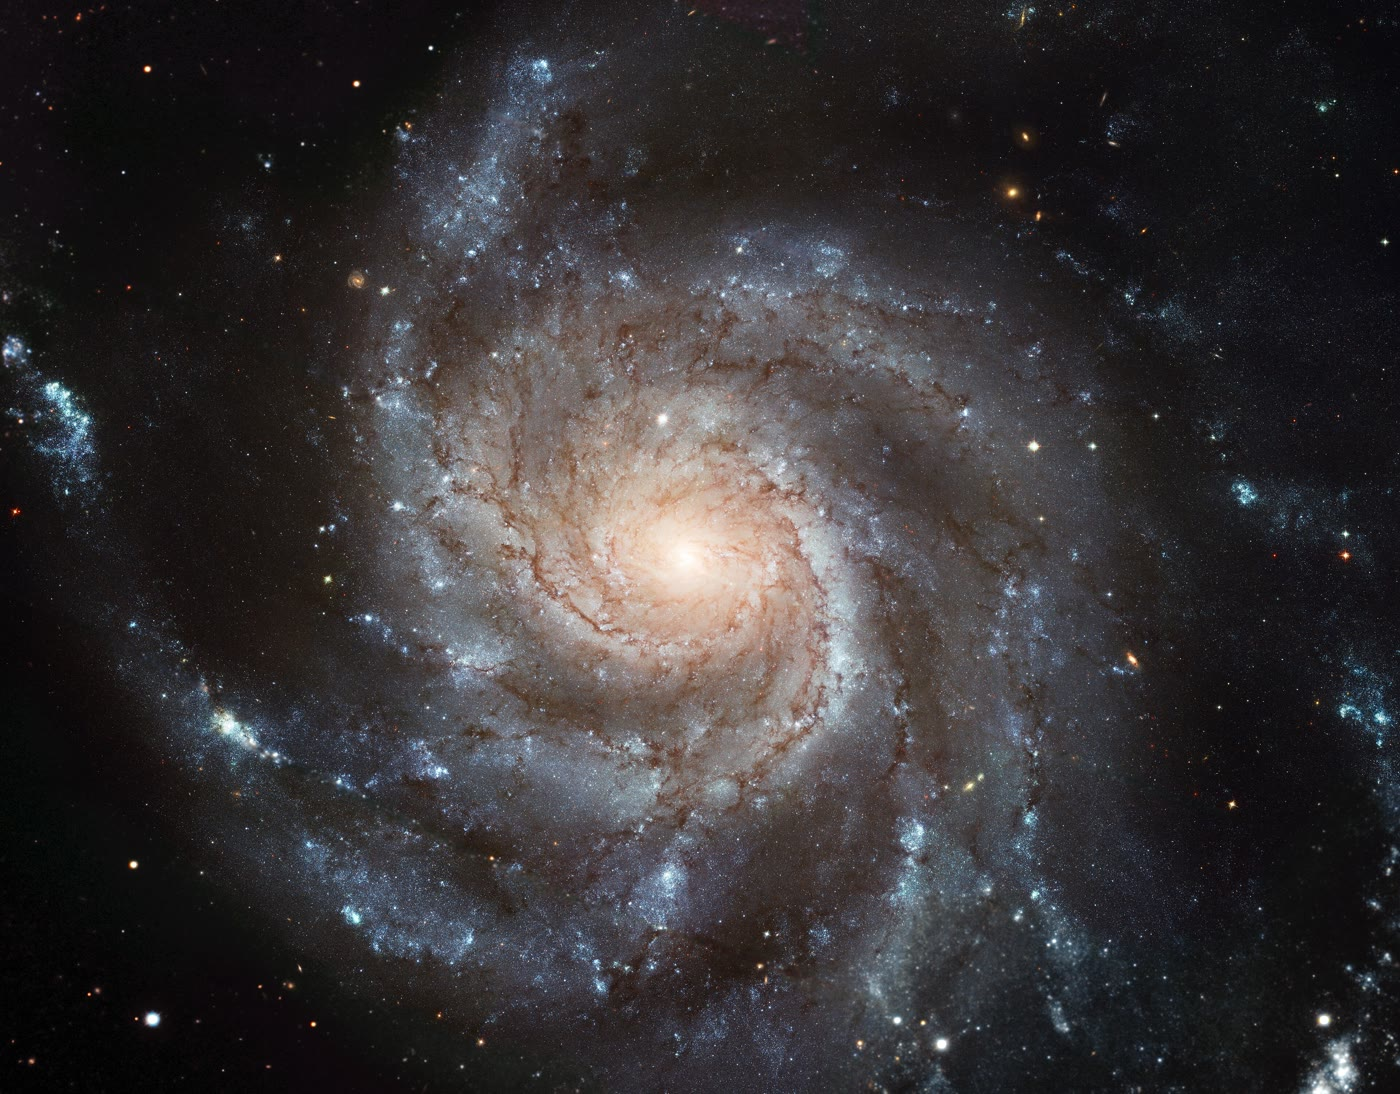
\includegraphics[width=0.66\linewidth]{images/book5/b3-m101.jpg}
\par\smallskip{\small हबल स्पेस टेलीस्कोप द्वारा सामने से देखी गई \omterm{def:b3:milky-way-galaxies:types}{सर्पिल मंदाकिनी} M101,
51 उद्भासनों का एक मोज़ेक, किनारों पर काटा हुआ: एक छोटा,
चमकीला, पीलापन लिए उभार; खुली भुजाएँ, अधिक नीली और युवा तारों के गुच्छों से गाँठदार;
भुजाओं के साथ-साथ भूरी धूल की पट्टियाँ। छवि: ESA और NASA
(Hubble, heic0602), CC BY~4.0.}\label{fig:b3:milky-way-galaxies:m101}
\end{omfigure}
% ledger: photo:b3-m101

सर्पिल भुजाएँ लिपटी हुई क्यों नहीं हैं? ऐसी चक्रिका में जिसका \omterm{def:b3:milky-way-galaxies:rotation-curve}{घूर्णन वक्र} समतल है,
केंद्र से आधी दूरी पर स्थित एक तारा आधे समय में एक चक्कर पूरा करता है।
तारों की एक सर्पिल हर फेरे में और कसती जाती, और चक्रिका के कुछ फेरों के बाद
वह एक कसी कुंडली बन जाती (\cref{exo:b3:milky-way-galaxies:11} देखिए)।

\begin{definition}[घनत्व-तरंग सिद्धांत]\label{def:b3:milky-way-galaxies:density-wave}
\emph{घनत्व-तरंग सिद्धांत}\index{घनत्व-तरंग सिद्धांत} सर्पिल भुजाओं को चक्रिका में
अधिक घनत्व की एक तरंग के रूप में समझाता है, एक ऐसा सर्पिल प्रारूप जो अपनी ही कोणीय चाल से,
जिसे प्रारूप-चाल कहते हैं, दृढ़तापूर्वक घूमता है, जबकि तारे और
गैस उसमें से होकर गुज़रते हैं, भीड़ वाली भुजा में प्रवेश करते समय धीमे पड़ते हैं और
उससे निकलते समय तेज़ हो जाते हैं, जैसे यातायात जाम में से गाड़ियाँ गुज़रती हैं।
\end{definition}

यह सिद्धांत, जिसे 1964 में प्रस्तावित किया गया, भुजाओं को लिपटने की समस्या से मुक्त करता है।
भुजा में प्रवेश करती गैस संपीड़ित होती है, और वहाँ तारे बनते हैं: भुजाएँ
युवा तारों और चमकती गैस से पहचानी जाती हैं, जबकि पुराने तारे कहीं अधिक समान रूप से फैले होते हैं।
क्या भुजाएँ दीर्घजीवी तरंगें हैं, यह अब भी विवादित है;
चक्रिकाओं के कंप्यूटर अनुकरण प्रायः ऐसी भुजाएँ उगाते हैं जो क्षणिक होती हैं,
जो घुलती और पुनः बनती हैं, और कोई गुज़रती मंदाकिनी या पट्टी
दो-भुजाओं वाले सर्पिल को प्रेरित कर सकती है।
% ledger: dobbs14:density-wave

\begin{definition}[अतिद्रव्यमान कृष्ण विवर]\label{def:b3:milky-way-galaxies:smbh}
एक \emph{अतिद्रव्यमान कृष्ण विवर}\index{अतिद्रव्यमान कृष्ण विवर} किसी मंदाकिनी के केंद्र में स्थित
दस लाख या उससे अधिक सौर द्रव्यमान वाला कृष्ण विवर होता है।
\end{definition}

आकाशगंगा के केंद्र में, संहत रेडियो स्रोत सैजिटेरियस~A*
तारों के बीच कसी और तेज़ कक्षाओं में स्थित है। इन कक्षाओं के लिए
लगभग चार मिलियन सूर्यों के बराबर केंद्रीय द्रव्यमान चाहिए, $\num[separate-uncertainty=true]{4.2 \pm 0.2 e6}$
सौर द्रव्यमान, मापनों की एक समीक्षा में। सैजिटेरियस~A* दूर की मंदाकिनियों के सापेक्ष
मुश्किल से गति करता है: सूर्य की कक्षा हटाने पर इसकी अवशिष्ट गति
अधिक से अधिक कुछ किलोमीटर प्रति सेकंड है, इसलिए यह उस द्रव्यमान का
कम से कम एक चौथाई धारण करता है। इसका आकार इसकी श्वार्ज़शिल्ड
त्रिज्या के तुल्य है, और इसका घनत्व, जो प्रति घन पारसेक \num{4e23} सौर द्रव्यमान से ऊपर है,
कृष्ण विवर से अपेक्षित घनत्व के बहुत निकट है: यह प्रमाण इतना प्रबल है कि
सैजिटेरियस~A* के कृष्ण विवर होने में कोई संदेह नहीं रहता।
% ledger: reid20:sgra, bhg16:structure, gravity19:r0

\begin{definition}[स्थानीय समूह; मंदाकिनी गुच्छ]\label{def:b3:milky-way-galaxies:groups}
\emph{स्थानीय समूह}\index{स्थानीय समूह} मंदाकिनियों का वह गुरुत्वाकर्षण से बद्ध समूह है
जिस पर आकाशगंगा और एंड्रोमेडा का प्रभुत्व है, और इनमें से प्रत्येक के अपने उपग्रह मंदाकिनियाँ हैं।
\emph{मंदाकिनी गुच्छ}\index{मंदाकिनी गुच्छ} गुरुत्वाकर्षण से बद्ध सबसे बड़े तंत्रों में से एक है:
इसमें अनेक मंदाकिनियाँ होती हैं, जो एक गर्म गैस के साथ, जो X-किरणें उत्सर्जित करती है,
मुख्यतः अदीप्त द्रव्य के एक साझे गर्त में
बँधी रहती हैं।
\end{definition}

सूर्य से \qty{3}{Mpc} के भीतर सौ से अधिक मंदाकिनियाँ हैं, जिनमें से अधिकांश
बौनी हैं। बृहत मैगेलैनिक मेघ लगभग \qty{50}{kpc} पर है, और एंड्रोमेडा
\qty{783}{kpc} पर है और \qty{300}{km.s^{-1}} की गति से हमारी ओर आ रहा है, और समूह के बद्ध
सदस्य समूह के द्रव्यमान-केंद्र से लगभग \qty{1.06}{Mpc} के भीतर स्थित हैं,
आकाशगंगा और एंड्रोमेडा के बीच, जहाँ वे ब्रह्मांड के प्रसार से अलग हो जाते हैं।
इसका द्रव्यमान दो बड़ी मंदाकिनियों की एक-दूसरे की ओर गति से ज्ञात होता है,
जो \num{5e12} सौर द्रव्यमान की कोटि का है। एक विशाल \omterm{def:b3:milky-way-galaxies:groups}{मंदाकिनी गुच्छ} में,
गर्म गैस, जिसका तापमान लगभग \qty{e8}{K} है, तारों के द्रव्यमान का लगभग दस गुना
द्रव्यमान रखती है; मंदाकिनियाँ और गैस मिलाकर भी गुरुत्वाकर्षण गर्त की गहराई के लिए
बहुत हल्की हैं, और गुच्छ का अधिकांश द्रव्यमान, जो
\num{e15} सौर द्रव्यमान की कोटि का है, अदीप्त है।
% ledger: mcconn12:local-group, kravtsov12:clusters

\section{दूरी सोपान}\label{sec:b3:milky-way-galaxies:ladder}

लंबन केवल ज्यामिति से दूरी देता है, परंतु लंबन दूरी के साथ
घटते हैं। इनका सबसे अच्छा सूचीपत्र उन तारों का लंबन मापता है, जो परिमाण~15 से चमकीले हैं,
जिसकी अनिश्चितता 0.02 से \qty{0.03}{mas} तक है, इसलिए
लगभग \qty{4}{kpc} तक \qty{10}{\percent} की दूरी प्राप्त होती है; बृहत मैगेलैनिक मेघ,
जो \qty{50}{kpc} पर है, का लंबन \qty{0.02}{mas} है।
इससे आगे दूरियाँ उन वस्तुओं पर टिकती हैं, जिनकी
दीप्ति ज्ञात है।
% ledger: gaia:dr3, freedman19:trgb

\begin{definition}[मानक मोमबत्ती; दूरी सोपान]\label{def:b3:milky-way-galaxies:ladder}
\emph{मानक मोमबत्ती}\index{मानक मोमबत्ती} वस्तुओं का ऐसा वर्ग है
जिनका निरपेक्ष कांति ज्ञात है, या जिसे दूरी से स्वतंत्र रूप से मापे गए किसी गुण से निकाला जा सकता है,
ताकि उसकी दृश्य कांति उसका दूरी-मापांक दे सके।
\emph{दूरी सोपान}\index{दूरी सोपान} उन विधियों की वह शृंखला है,
जिसकी प्रत्येक विधि उन वस्तुओं पर अंशांकित होती है, जो इतनी निकट हों कि
पिछली विधि से भी मापी जा सकें, और जो लंबनों से दूरियाँ
विस्तारित ब्रह्मांड तक ले जाती है।
\end{definition}

\begin{definition}[सीफ़ीड परिवर्ती; लेविट नियम]\label{def:b3:milky-way-galaxies:cepheid}
\emph{सीफ़ीड परिवर्ती}\index{सीफ़ीड परिवर्ती} एक युवा, दीप्तिमान,
स्पंदनशील तारा है, जिसकी चमक सख़्ती से नियमित आवर्त काल के साथ बदलती है,
लगभग एक दिन से लेकर कई सप्ताह तक। \emph{लेविट नियम}\index{लेविट नियम},
या आवर्त--दीप्ति संबंध, सीफ़ीड के माध्य निरपेक्ष कांति और उसके आवर्त के लघुगणक के बीच
का रैखिक संबंध है, जिसमें अधिक दीप्तिमान तारों के
आवर्त लंबे होते हैं।
\end{definition}

1908 में लघु मैगेलैनिक मेघ में यह संबंध खोजा गया, जिसके तारे
लगभग एक ही दूरी पर हैं। जिस मंदाकिनी में सीफ़ीड होता है, उसकी धूल
उसे मंद और लाल कर देती है; परंतु मंदन दृश्य प्रकाश में निकट अवरक्त से अधिक होता है,
और किसी दिए गए प्रकार की धूल के लिए इसका अनुपात स्थिर रहता है, और I और V बैंडों के परिमाणों का संयोजन $W_I = I - 1.55\,(V - I)$, जिसे
वेसेनहाइट सूचकांक कहते हैं, और इसे इस प्रकार चुना जाता है कि मंदन
निरस्त हो जाए। नीचे का चित्र बृहत मैगेलैनिक मेघ के 2315 सीफ़ीडों के लिए यह दिखाता है:
\omterm{def:b3:milky-way-galaxies:cepheid}{लेविट नियम} एक कसी हुई रेखा है, जिसका प्रकीर्णन
\qty{0.078}{mag} है, अर्थात एक ही तारे के लिए दूरी में

\qty{3.6}{\percent} है।
% ledger: sos15:leavitt, data:b5-ogle-lmc-cep

\begin{omfigure}
\centering
\begin{tikzpicture}
\begin{axis}[width=0.80\linewidth, height=0.52\linewidth,
  xmin=-0.05, xmax=1.6, ymin=10, ymax=16.6, y dir=reverse,
  xlabel={$\log_{10}(P/\mathrm{d})$}, ylabel={वेसेनहाइट सूचकांक $W_I$ (mag)},
  tick label style={font=\scriptsize}, label style={font=\small},
  legend style={font=\scriptsize, at={(0.5,-0.17)}, anchor=north, legend columns=3, draw=none, cells={anchor=west}, /tikz/every even column/.append style={column sep=1em}},
  legend image post style={scale=2.2}]
\addplot[only marks, mark=*, mark size=0.45pt, omDef, opacity=0.6] table[x=logp, y=w] {figdata/out/bachelor-3-distance_ladder-pl.dat};
\addlegendentry{सीफ़ीड}
\addplot[only marks, mark=x, mark size=1.6pt, red!70!black] table[x=logp, y=w] {figdata/out/bachelor-3-distance_ladder-clipped.dat};
\addlegendentry{अलग रखे गए ($>3\sigma$)}
\addplot[thick, black] table[x=logp, y=w_fit] {figdata/out/bachelor-3-distance_ladder-fit.dat};
\addlegendentry{फ़िट}
\node[font=\scriptsize, anchor=south west, fill=white, inner sep=1pt] at (axis cs:0.55,11.0) {$W_I = -3.315\log_{10}P + 15.889$};
\end{axis}
\end{tikzpicture}
\par\smallskip{\small बृहत मैगेलैनिक मेघ में \omterm{def:b3:milky-way-galaxies:cepheid}{लेविट नियम}:
मूल विधा में स्पंदन करने वाले 2315 सीफ़ीडों का वेसेनहाइट सूचकांक
उनके आवर्त के लघुगणक के विरुद्ध (OGLE सर्वेक्षण, सोसिन्स्की और
अन्य, 2015, CDS के माध्यम से)। चमकीले तारे ऊपर हैं। न्यूनतम वर्ग से फ़िट की गई
एक सीधी रेखा, उससे तीन मानक विचलनों से अधिक दूर के 92 तारों को अलग रखने के बाद,
प्रकाशित संबंध ($-3.314$, $15.888$) को पुनः उत्पन्न करती है।
मेघ की दूरी-मापांक 18.477 के साथ, यह रेखा
किसी भी सीफ़ीड का निरपेक्ष वेसेनहाइट कांति उसके आवर्त से दे देती है।}\label{fig:b3:milky-way-galaxies:leavitt}
\end{omfigure}
% ledger: data:b5-ogle-lmc-cep, sos15:leavitt, freedman19:trgb

\begin{definition}[लाल दानव शाखा का शीर्ष]\label{def:b3:milky-way-galaxies:trgb}
\emph{लाल दानव शाखा का शीर्ष}\index{लाल दानव शाखा का शीर्ष}
(TRGB) किसी पुराने \omterm{def:b3:milky-way-galaxies:populations}{तारकीय समष्टि} के लाल दानवों की दीप्तियों की
तीखी ऊपरी सीमा है, जिसे उनके क्रोड में हीलियम के प्रज्वलन से तय किया जाता है,
यानी हीलियम फ़्लैश; I बैंड में यह हर पुरानी समष्टि में लगभग एक ही निरपेक्ष
कांति पर होती है, जो $M_I \approx -4.05$ है और वर्ण $V - I = 1.6$ पर मापी जाती है,
और जो रासायनिक संघटन पर केवल कमज़ोर रूप से निर्भर करती है।
\end{definition}

यह शीर्ष मंदाकिनियों के विरल तारकीय प्रभामंडलों में मापा जाता है, जहाँ
धूल कम होती है और भीड़ भी कम; यह पुराने प्रभामंडल तारों का उपयोग करता है, जहाँ सीफ़ीड
युवा चक्रिका तारों का उपयोग करते हैं, और दोनों विधियाँ कोई भौतिकी साझा नहीं करतीं। सीफ़ीड और
TRGB कुछ दर्जन मेगापारसेक तक पहुँचते हैं, उन मंदाकिनियों तक जहाँ एक दुर्लभ और
कहीं अधिक चमकीली \omterm{def:b3:milky-way-galaxies:ladder}{मानक मोमबत्ती} विस्फोट कर चुकी है: टाइप~Ia अधिनवतारा, जो एक श्वेत वामन का
तापनाभिकीय विस्फोट है, जैसा भौतिकी की पुस्तकों में स्मरण कराया गया है,
जिसकी शिखर निरपेक्ष कांति, प्रकाश-वक्र के आकार और अपने वर्ण के लिए सुधार करने के बाद,
इतनी होती है:
$M_B = \qty[separate-uncertainty=true]{-19.253 \pm 0.027}{mag}$।
ऐसे अधिनवतारे सैकड़ों मेगापारसेक तक देखे जाते हैं।
% ledger: freedman19:trgb, riess22:h0

\begin{definition}[टली--फ़िशर संबंध]\label{def:b3:milky-way-galaxies:tully-fisher}
\emph{टली--फ़िशर संबंध}\index{टली--फ़िशर संबंध} एक \omterm{def:b3:milky-way-galaxies:types}{सर्पिल मंदाकिनी} की
दीप्ति, या बेहतर रूप से तारों और गैस के द्रव्यमान, और
उसके सपाट \omterm{def:b3:milky-way-galaxies:rotation-curve}{घूर्णन वक्र} की चाल के बीच का सहसंबंध है; बैरियोनिक रूप में,
$M_\mathrm{b} = A\,V^4$, यह लगभग 30 से
\qty{300}{km.s^{-1}} तक लागू होता है।
\end{definition}

मंदाकिनी का 21-cm स्पेक्ट्रम उसकी अधिकतम घूर्णन चाल देता है; यह संबंध
उसकी दीप्ति उसकी दूरी से स्वतंत्र रूप से देता है, और उसका फ़्लक्स
फिर दूरी देता है: यह उन सर्पिल मंदाकिनियों के लिए एक पायदान है जो
एकल तारों के लिए बहुत दूर हैं। आकाशगंगा अपनी दीप्ति और घूर्णन के आधार पर इस संबंध पर ठीक बैठती है।
% ledger: mcgaugh00:btf, nrao:hi-line, bhg16:structure

\begin{omfigure}
\centering
\pgfplotstableread{figdata/out/bachelor-3-distance_ladder-ladder.dat}\laddertab
\pgfplotstableread{figdata/out/bachelor-3-distance_ladder-anchors.dat}\anchortab
\pgfplotstablegetelem{0}{d_hi}\of{\laddertab}\let\plxhi\pgfplotsretval
\pgfplotstablegetelem{1}{d_lo}\of{\laddertab}\let\cephlo\pgfplotsretval
\pgfplotstablegetelem{1}{d_hi}\of{\laddertab}\let\cephhi\pgfplotsretval
\pgfplotstablegetelem{3}{d_lo}\of{\laddertab}\let\snlo\pgfplotsretval
\pgfplotstablegetelem{3}{d_hi}\of{\laddertab}\let\snhi\pgfplotsretval
\pgfplotstablegetelem{1}{d}\of{\anchortab}\let\mthirtyone\pgfplotsretval
\pgfplotstablegetelem{2}{d}\of{\anchortab}\let\nfourtwo\pgfplotsretval
\begin{tikzpicture}
\begin{axis}[width=0.92\linewidth, height=0.42\linewidth,
  xmode=log, xmin=1e-3, xmax=2e6, ymin=0.4, ymax=4.9,
  ytick={1,2,3,4}, yticklabels={लंबन, सीफ़ीड, TRGB, SNe~Ia},
  xtick={1e-3,1e-2,1e-1,1,10,100,1e3,1e4,1e5,1e6},
  xticklabels={1~pc,,,1~kpc,,,1~Mpc,,,1~Gpc},
  xlabel={दूरी}, tick label style={font=\scriptsize}, label style={font=\small},
  y tick label style={font=\small}, axis y line*=left, axis x line*=bottom]
\draw[line width=7pt, omDef!70] (axis cs:1e-3,1) -- (axis cs:\plxhi,1);
\draw[line width=7pt, omMeth!70] (axis cs:\cephlo,2) -- (axis cs:\cephhi,2);
\draw[line width=7pt, omProp!70] (axis cs:\cephlo,3) -- (axis cs:\cephhi,3);
\draw[line width=7pt, red!60] (axis cs:\snlo,4) -- (axis cs:\snhi,4);
\draw[densely dotted, thick] (axis cs:\cephlo,0.4) -- (axis cs:\cephlo,4.55) node[anchor=south, font=\scriptsize] {LMC};
\draw[densely dotted, thick] (axis cs:\mthirtyone,0.4) -- (axis cs:\mthirtyone,4.55) node[anchor=south, font=\scriptsize] {M31};
\draw[densely dotted, thick] (axis cs:\nfourtwo,0.4) -- (axis cs:\nfourtwo,4.55) node[anchor=south, font=\scriptsize] {NGC~4258};
\draw[->, thick, black!60] (axis cs:\plxhi,1.25) to[out=30, in=200] (axis cs:\cephlo,1.75);
\draw[->, thick, black!60] (axis cs:\cephhi,2.25) to[out=40, in=220] (axis cs:\snlo,3.75);
\end{axis}
\end{tikzpicture}
\par\smallskip{\small \omterm{def:b3:milky-way-galaxies:ladder}{दूरी सोपान} के पायदान, साथ में वे दूरियाँ जिन पर यहाँ हर एक का उपयोग हुआ है:
सबसे अच्छे कैटलॉग के लंबन, \qty{4}{kpc} तक, \qty{10}{\percent} तक की त्रुटि पर;
सीफ़ीड और TRGB बृहत मैगेलैनिक मेघ से लेकर निकटतम टाइप~Ia अधिनवतारों के
मेज़बान मंदाकिनियों तक, \qty{45}{Mpc} तक;
सुचारु प्रसार के अधिनवतारे, रेडशिफ़्ट 0.023
से 0.15 तक (\qtyrange{96}{616}{Mpc} के बीच, $H_0 = 73$ के लिए)। बिंदीदार रेखाएँ:
सीफ़ीड पैमाने के दो एंकर, जो ज्यामितीय दूरियों वाले हैं (बृहत मैगेलैनिक मेघ में ग्रहण-द्विक तारे, और NGC~4258 के कृष्ण विवर की परिक्रमा करने वाले जल-मेसर),
और M31, जो सबसे निकटतम बड़ा सर्पिल है।
तीर: प्रत्येक पायदान उन वस्तुओं पर अंशांकित होता है, जिन्हें नीचे वाला पायदान भी
मापता है: आकाशगंगा के सीफ़ीड उनके लंबन से, निकट की मंदाकिनियों के अधिनवतारे
अपने मेज़बानों के सीफ़ीड और TRGB से
।}\label{fig:b3:milky-way-galaxies:ladder-rungs}
\end{omfigure}
% ledger: gaia:dr3, riess22:h0, freedman19:trgb, mcconn12:local-group

सोपान के शीर्ष पर अधिनवतारे ब्रह्मांड का प्रसार मापते हैं।
हबल का नियम, जैसा भौतिकी की पुस्तकों में स्मरण कराया गया है,
किसी दूर की मंदाकिनी के अपसरण वेग $cz$ को उसकी दूरी $d$ के समानुपाती
बनाता है, $cz = H_0 d$ छोटे रेडशिफ़्ट $z$ के लिए; हबल स्थिरांक $H_0$
ढलान है, और अधिनवतारे, अपनी सोपान से प्राप्त दूरियों के साथ, उसे देते हैं।

\begin{definition}[हबल तनाव]\label{def:b3:milky-way-galaxies:tension}
\emph{हबल तनाव}\index{हबल तनाव} वह असहमति है, जो \omterm{def:b3:milky-way-galaxies:ladder}{दूरी सोपान} से
स्थानीय रूप से मापे गए हबल स्थिरांक के मान और
कॉस्मिक माइक्रोवेव पृष्ठभूमि से मानक ब्रह्मांड-विज्ञान मॉडल के साथ
निकाले गए मान के बीच पाई जाती है।
\end{definition}

\begin{dated}{2022}
42 टाइप~Ia अधिनवतारों के मेज़बान मंदाकिनियों के सीफ़ीड, गाया लंबनों पर स्थिर किए गए,
NGC~4258 के मेसर और बृहत मैगेलैनिक मेघ के ग्रहण-द्विक तारे
देते हैं,
$H_0 = \qty[separate-uncertainty=true]{73.04 \pm 1.04}{km.s^{-1}.Mpc^{-1}}$।
\omterm{def:b3:milky-way-galaxies:trgb}{लाल दानव शाखा का शीर्ष}, लगभग सौ अधिनवतारों को अंशांकित करते हुए,
2019 में $H_0 = 69.8 \pm 0.8 \pm \qty{1.7}{km.s^{-1}.Mpc^{-1}}$ दिया
(सांख्यिकीय और व्यवस्थित)। प्लैंक उपग्रह का कॉस्मिक
माइक्रोवेव पृष्ठभूमि का मानचित्र, मानक ब्रह्मांड-विज्ञान मॉडल से पढ़ा जाने पर,
$H_0 = \qty[separate-uncertainty=true]{67.4 \pm 0.5}{km.s^{-1}.Mpc^{-1}}$ सूचित करता है।
सीफ़ीड का मान और पृष्ठभूमि का मान पाँच मानक
विचलनों से भिन्न हैं; TRGB का मान इन दोनों के बीच पड़ता है। इस असंगति का
स्रोत ज्ञात नहीं है: या तो किसी एक सोपान में अभी तक न खोजी गई त्रुटि,
या मॉडल में छूट गई भौतिकी।
\end{dated}
% ledger: riess22:h0, freedman19:trgb, planck18:h0

\begin{inthelab}[एक खगोलमितीय उपग्रह और उसका सूचीपत्र]
उपग्रह गैया एक निर्धारित प्रतिरूप में आकाश को स्कैन करता है, ताकि
मिशन के दौरान हर तारे को बार-बार मापा जाए। धरती पर, एक डेटा-प्रसंस्करण संघ की
समन्वय इकाइयाँ इन मापनों को
एक अरब से अधिक स्रोतों में से हर एक के लिए स्थिति, लंबन और उचित गति में बदलती हैं:
आकाश पर किसी तारे की छोटी गतियों में से
लंबन वह भाग है जो हर वर्ष दोहराता है, और उचित गति
वह भाग है जो संचित होता है। हर सूचीपत्र के साथ ऐसे शोधपत्र जारी होते हैं जो
उसके प्रसंस्करण और सत्यापन का वर्णन करते हैं, और इस खंड के चित्रों में हर दूरी
जो किसी लंबन पर आधारित है, वह ऐसे ही किसी
सूचीपत्र पर टिकी है।
\end{inthelab}

\begin{dated}{2022}
गैया का तीसरा सूचीपत्र, जो 13 जून 2022 को 34 महीनों के प्रेक्षणों से जारी हुआ,
लगभग 1.46~अरब स्रोतों के लिए स्थिति, लंबन और उचित गति,
परिमाण~3 से~21 तक के, और 33~मिलियन तारों के लिए माध्य त्रिज्य वेग देता है।
इसकी लंबन अनिश्चितताएँ 0.02 से
\qty{0.03}{mas} तक, परिमाण~15 से चमकीले तारों के लिए, \qty{0.07}{mas}
परिमाण~17 पर, और \qty{0.5}{mas} परिमाण~20 पर हैं।
\end{dated}
% ledger: gaia:dr3

\section{अभ्यास}

\begin{exercise}[$\star$]\label{exo:b3:milky-way-galaxies:1}
सूर्य का मंदाकिनीय वर्ष। (क)~$R_0 = \qty{8.178}{kpc}$ और
$V_0 = \qty{229}{km.s^{-1}}$ लेकर, मंदाकिनीय केंद्र के परितः सूर्य की कक्षा का आवर्तकाल
मिलियन वर्षों में परिकलित कीजिए। (ख)~सौरमंडल बनने के बाद से, जो
\qty{4.54}{Gyr} पहले हुआ, सूर्य कितनी बार परिक्रमा कर चुका है?
\end{exercise}

\begin{exercise}[$\star$]\label{exo:b3:milky-way-galaxies:2}
सैजिटेरियस~A* की प्रतिक्षेप गति। (क)~\qty{1}{mas} प्रति वर्ष की उचित गति
\qty{1}{kpc} पर \qty{1}{au} प्रति वर्ष की अनुप्रस्थ चाल है: इसे व्यक्त कीजिए
किलोमीटर प्रति सेकंड में। (ख)~मान लीजिए सैजिटेरियस~A* मंदाकिनीय केंद्र पर,
\qty{8.178}{kpc} की दूरी पर, विराम अवस्था में है, और मंदाकिनीय समतल के अनुदिश
\qty{6.411}{mas} प्रति वर्ष बहता है। केंद्र के परितः सूर्य की चाल परिकलित कीजिए और उसकी तुलना
समीक्षा के मान \qty[separate-uncertainty=true]{248 \pm 3}{km.s^{-1}} से कीजिए। (ग)~घूर्णन की दिशा में सूर्य की
विशिष्ट गति, \qty{11}{km.s^{-1}}, घटाइए
और \omterm{def:b3:milky-way-galaxies:rotation-curve}{घूर्णन वक्र} के $V_0$ से तुलना कीजिए।
\end{exercise}

\begin{exercise}[$\star$]\label{exo:b3:milky-way-galaxies:3}
दीर्घवृत्तीय मंदाकिनियों का वर्गीकरण। (क)~एक \omterm{def:b3:milky-way-galaxies:types}{दीर्घवृत्तीय मंदाकिनी} की समप्रकाश-रेखाओं का
अक्ष-अनुपात 0.6 है: उसका वर्ग बताइए। (ख)~E7 का अक्ष-अनुपात क्या होता है?
(ग)~E0 मंदाकिनी एक चपटी संरचना क्यों हो सकती है?
\end{exercise}

\begin{exercise}[$\star$]\label{exo:b3:milky-way-galaxies:4}
लंगर। बृहत् मैगेलैनिक मेघ की दूरियाँ
($\mu = 18.477$), एंड्रोमेडा ($\mu = 24.47$) और NGC~4258
($\mu = 29.398$) की दूरियाँ परिकलित कीजिए। मेघ के किसी तारे का लंबन क्या होगा, और मेघ
की दूरी लंबनों से क्यों नहीं मापी जा सकती?
\end{exercise}

\begin{exercise}[$\star\star$]\label{exo:b3:milky-way-galaxies:5}
\omterm{def:b3:milky-way-galaxies:rotation-curve}{ऊर्ट स्थिरांक} $A = \qty{15.3}{km.s^{-1}.kpc^{-1}}$ और
$B = \qty{-11.9}{km.s^{-1}.kpc^{-1}}$ से: (क)~LSR की कोणीय चाल परिकलित कीजिए
और $R_0 = \qty{8.178}{kpc}$ लेकर वृत्तीय वेग $V_0$ परिकलित कीजिए;
(ख)~सूर्य पर \omterm{def:b3:milky-way-galaxies:rotation-curve}{घूर्णन वक्र} की प्रवणता परिकलित कीजिए। (ग)~इसकी तुलना
लाल दानवों के \omterm{def:b3:milky-way-galaxies:rotation-curve}{घूर्णन वक्र} ($V_0 = \qty{229.0}{km.s^{-1}}$,
प्रवणता \qty{-1.7}{km.s^{-1}} प्रति किलोपारसेक) से कीजिए और सुझाइए कि दोनों
भिन्न क्यों हैं, यह देखते हुए कि उसी माप में $C$ और $K$ शून्येतर पाए गए।
\end{exercise}

\begin{exercise}[$\star\star$]\label{exo:b3:milky-way-galaxies:6}
एक समतल \omterm{def:b3:milky-way-galaxies:rotation-curve}{घूर्णन वक्र} और स्थानीय घनत्व। (क)~गोलीय मंदाकिनी के लिए, जिसका
\omterm{def:b3:milky-way-galaxies:rotation-curve}{घूर्णन वक्र} \qty{229}{km.s^{-1}} पर समतल है, घनत्व परिकलित कीजिए
\qty{8.178}{kpc} पर, सौर द्रव्यमान प्रति घन पारसेक में
($G = \qty{4.301e-6}{kpc.(km.s^{-1})^2}$ प्रति सौर द्रव्यमान)। (ख)~दिखाइए
कि एक सौर द्रव्यमान प्रति घन पारसेक \qty{37.96}{GeV.cm^{-3}} के बराबर है, और
स्थानीय अदीप्त-द्रव्य घनत्व, \qty{0.30}{GeV.cm^{-3}}, को सौर द्रव्यमान प्रति घन पारसेक में
व्यक्त कीजिए। (ग)~(क) का घनत्व बड़ा क्यों है?
\end{exercise}

\begin{exercise}[$\star\star$]\label{exo:b3:milky-way-galaxies:7}
एक सीफ़ीड दूरी। एक काल्पनिक \omterm{def:b3:milky-way-galaxies:types}{सर्पिल मंदाकिनी} में आवर्तकाल
\qty{30}{d} वाला एक सीफ़ीड है, जिसका माध्य वेसेनहाइट सूचकांक $W_I = \qty{25.00}{mag}$ है।
(क)~बृहत् मैगेलैनिक मेघ के \omterm{def:b3:milky-way-galaxies:cepheid}{लेविट नियम} का उपयोग करके,
$W_I = -3.314\log_{10}P + 15.888$, और मेघ के दूरी-मापांक
18.477 से, सीफ़ीड का निरपेक्ष वेसेनहाइट परिमाण परिकलित कीजिए। (ख)~मंदाकिनी की
दूरी परिकलित कीजिए। (ग)~नियम का प्रकीर्णन \qty{0.077}{mag} है: एक सीफ़ीड से
और पचास सीफ़ीडों से सापेक्ष दूरी त्रुटि क्या है?
\end{exercise}

\begin{exercise}[$\star\star$]\label{exo:b3:milky-way-galaxies:8}
एक TRGB दूरी। एक काल्पनिक मंदाकिनी के प्रभामंडल में \omterm{def:b3:milky-way-galaxies:trgb}{लाल दानव शाखा का
शीर्ष} $I = \qty{26.00}{mag}$ पर मिलता है; दृष्टि-रेखा के अनुदिश धूल I बैंड को
\qty{0.05}{mag} से मंद करती है। $M_I = -4.05$ लेकर, दूरी-मापांक और दूरी
परिकलित कीजिए। शीर्ष की \qty{0.04}{mag} की अनिश्चितता
दूरी में क्या अर्थ रखती है?
\end{exercise}

\begin{exercise}[$\star\star$]\label{exo:b3:milky-way-galaxies:9}
अधिनवतारों से हबल स्थिरांक। सुचारु प्रसार वाले एक अधिनवतारा के लिए,
$\log_{10}(cz) - 0.2\,m_B = a_B$, जो अधिनवतारों के हबल आरेख का अंतःखंड है, और
दूरी-मापांक $m_B - M_B = 5\log_{10}(d/\mathrm{Mpc}) + 25$ है। (क)~दिखाइए
कि $\log_{10}H_0 = 0.2\,M_B + a_B + 5$ ($H_0$ किलोमीटर प्रति सेकंड
प्रति मेगापारसेक में)। (ख)~$M_B = -19.253$ और $a_B = 0.714158$ लेकर
$H_0$ परिकलित कीजिए। (ग)~कौन-सा $M_B$ $H_0 = \qty{67.4}{km.s^{-1}.Mpc^{-1}}$ देगा?
कितने परिमाणों से,
और दूरियों के कितने भिन्नांश से,
ये दोनों अंशांकन भिन्न हैं?
\end{exercise}

\begin{exercise}[$\star\star\star$]\label{exo:b3:milky-way-galaxies:10}
टली--फ़िशर नियम कहाँ से आता है। (क)~द्रव्यमान $M$ की एक चक्रिका-मंदाकिनी
त्रिज्या $R$ है और $V$ से घूमती है: दिखाइए कि $M \approx RV^2/G$। (ख)~यदि सभी
सर्पिल मंदाकिनियों का माध्य पृष्ठ घनत्व $\Sigma = M/(\pi R^2)$ एक ही हो,
तो दिखाइए कि $M \propto V^4$। (ग)~एक ही बैरिऑनिक संबंध पर स्थित दो काल्पनिक मंदाकिनियाँ
100 और \qty{229}{km.s^{-1}} पर घूमती हैं: उनके द्रव्यमानों का अनुपात क्या है?
(घ)~दो मंदाकिनियाँ एक ही चाल से घूमती हैं और उनकी दीप्ति समान है;
एक का फ़्लक्स दूसरे का चार गुना है। उनकी
दूरियों की तुलना कीजिए।
\end{exercise}

\begin{exercise}[$\star\star\star$]\label{exo:b3:milky-way-galaxies:11}
कुंडलन समस्या। एक चक्रिका समतल खंड वाले वक्र के साथ
\qty{229}{km.s^{-1}} पर घूमती है। (क)~इस चाल को किलोपारसेक प्रति
अरब वर्ष में बदलिए। (ख)~शून्य समय पर तारों की एक सीधी भुजा 4 से
\qty{12}{kpc} तक फैली है। दोनों सिरों पर कक्षीय आवर्तकाल परिकलित कीजिए। (ग)~
\qty{1}{Gyr} के बाद, उसका भीतरी सिरा अपने बाहरी सिरे से किस कोण से आगे बढ़ गया है?
यह सर्पिल के कितने चक्कर के बराबर है, और भुजा कैसी दिखेगी?
(घ)~घनत्व-तरंग इससे कैसे बचती है?
\end{exercise}

\begin{exercise}[$\star\star\star$]\label{exo:b3:milky-way-galaxies:12}
केंद्र पर स्थित कृष्ण विवर। केंद्रीय द्रव्यमान को
\num{4.2e6} सौर द्रव्यमान और $R_0 = \qty{8178}{pc}$ मान लीजिए। (क)~तारा S2
इसकी परिक्रमा \num{16}~वर्ष में करता है: उसकी कक्षा का अर्ध-दीर्घ अक्ष
खगोलीय इकाइयों में (सौर इकाइयों में केप्लर का तीसरा नियम, $a^3 = MP^2$ जिसमें
$a$ au में, $P$ वर्षों में और $M$ सौर द्रव्यमानों में है) और उसका कोणीय आकार
पृथ्वी से देखा गया परिकलित कीजिए। (ख)~कृष्ण विवर की श्वार्ट्सचाइल्ड त्रिज्या
मीटर में और खगोलीय इकाइयों में, तथा पृथ्वी से उसके व्यास द्वारा अंतरित कोण,
माइक्रोआर्कसेकंड में परिकलित कीजिए। (ग)~इसकी श्वार्ट्सचाइल्ड त्रिज्या के भीतर
द्रव्यमान का माध्य घनत्व, सौर द्रव्यमान प्रति घन
पारसेक में, परिकलित कीजिए, और उसकी तुलना सैजिटेरियस~A* की गति द्वारा निर्धारित
निम्न सीमा से कीजिए, जो \num{4e23} सौर द्रव्यमान प्रति घन पारसेक है।
\end{exercise}

\section{समस्या: आकाशगंगा का द्रव्यमान मापना}

\begin{problem}[{सप्ताहांत समस्या --- तारों और गैस की गतियों से
\qty{20}{kpc} के भीतर के अदीप्त द्रव्य तक}]
\label{pb:b3:milky-way-galaxies:1}
मान लीजिए $R_0 = \qty{8.18}{kpc}$ और $G = \qty{4.301e-6}{kpc.(km.s^{-1})^2}$ प्रति
सौर द्रव्यमान, और \qty{4.74}{km.s^{-1}} उस उचित गति के लिए जो
\qty{1}{kpc} पर \qty{1}{mas} प्रति वर्ष है। सभी वेगें
LSR के सापेक्ष हैं। अध्याय के ऊर्ट और स्पर्शबिंदु प्रमेयों का, और
गतिकीय द्रव्यमानों के लिए गोलीय सन्निकटन $M = RV^2/G$ का उपयोग कीजिए।

\medskip\noindent\textbf{भाग I --- स्थानीय घूर्णन।} लाल-क्लंप तारों का एक काल्पनिक
सर्वेक्षण, जो सभी $d = \qty{1.00}{kpc}$ दूरी पर मंदाकिनीय समतल में हैं,
माध्य अरीय वेग देता है: $\ell = \ang{45}$ पर \qty{+15.4}{km.s^{-1}} और
$\ell = \ang{135}$ पर \qty{-15.2}{km.s^{-1}}, तथा
देशांतर में माध्य उचित गतियाँ $\ell = \ang{90}$ पर \qty{-5.91}{mas} प्रति वर्ष
और $\ell = \ang{0}$ पर \qty{+0.55}{mas} प्रति वर्ष।
\begin{enumerate}
\item ऊर्ट का सूत्र अरीय वेगों का क्या पूर्वानुमान देता है
  $\ell = \ang{45}$, \ang{90}, \ang{135} और \ang{180} पर?
\item दो अरीय वेगों से $A$ परिकलित कीजिए।
\item $B$ को $\ell = \ang{90}$ पर उचित गति से परिकलित कीजिए।
\item $B$ को $\ell = \ang{0}$ पर उचित गति से फिर से परिकलित कीजिए, और
  तुलना कीजिए।
\item LSR की कोणीय चाल और वृत्तीय वेग
  $V_0$ परिकलित कीजिए।
\item सूर्य पर \omterm{def:b3:milky-way-galaxies:rotation-curve}{घूर्णन वक्र} की प्रवणता परिकलित कीजिए। क्या वक्र
  बढ़ता, समतल खंड या घटता है?
\item सूर्य की कक्षा का आवर्तकाल और
  \qty{4.54}{Gyr} में परिभ्रमणों की संख्या परिकलित कीजिए।
\end{enumerate}

\medskip\noindent\textbf{भाग II --- आंतरिक घूर्णन वक्र।} मान लीजिए
$V_0 = \qty{229}{km.s^{-1}}$। 21-cm प्रोफ़ाइलों में सबसे ऊँचे अरीय वेग
$\ell = \ang{40}$, \ang{50}, \ang{60} और \ang{70} पर
82.9, 55.6, 32.4 और \qty{14.9}{km.s^{-1}} हैं।
\begin{enumerate}[resume]
\item स्पर्शबिंदु विधि को $\ang{0} < \ell < \ang{90}$ की आवश्यकता क्यों होती है
  (या उसका दर्पण चतुर्थांश), और यह सौर वृत्त से परे क्यों विफल हो जाती है?
\item प्रत्येक देशांतर के लिए स्पर्शबिंदु की त्रिज्या परिकलित कीजिए।
\item प्रत्येक स्पर्शबिंदु पर $V(R)$ परिकलित कीजिए।
\item किलोहर्ट्ज़ में, $\ell = \ang{40}$ के स्पर्शबिंदु पर गैस की रेखा अपनी
  विराम आवृत्ति \qty{1420.405751}{MHz} से कितनी विस्थापित है,
  और किस दिशा में?
\item लाल दानव वक्र से तुलना कीजिए, जो \qty{5.27}{kpc} पर \qty{226.8}{km.s^{-1}} देता है,
  और \qty{7.22}{kpc} पर \qty{229.6}{km.s^{-1}} देता है। क्या आंतरिक
  वक्र बढ़ता, समतल खंड या घटता है?
\item यदि $\ell = \ang{40}$ के स्पर्शबिंदु पर चाल उस केंद्रीय बिंदु-द्रव्यमान की होती
  जो सूर्य को $V_0$ पर धारण करता है, तो वह कितनी होती?
  यह तुलना द्रव्यमान के वितरण के बारे में क्या बताती है?
\end{enumerate}

\medskip\noindent\textbf{भाग III --- दृश्य द्रव्यमान।} अध्याय के द्रव्यमान मॉडल का उपयोग कीजिए,
सौर द्रव्यमान और किलोपारसेक इकाइयों में: एक
प्लमर उभार $M = \num{1.067e10}$, $b = 0.3$; एक पतली मियामोतो--नागाई चक्रिका
$M = \num{3.944e10}$, $a = 5.3$, $b = 0.25$; उसी द्रव्यमान की एक \omterm{def:b3:milky-way-galaxies:structure}{मोटी चक्रिका},
जिसके $a = 2.6$, $b = 0.8$ हैं।
\begin{enumerate}[resume]
\item मॉडल का कुल दृश्य द्रव्यमान परिकलित कीजिए और उसकी तुलना
  आकाशगंगा के तारकीय द्रव्यमान के समीक्षा-मान, \qty[separate-uncertainty=true]{5 \pm 1 e10}{}
  सौर द्रव्यमान से कीजिए।
\item \qty{20}{kpc} पर केवल उभार का वृत्तीय वेग परिकलित कीजिए।
\item \qty{20}{kpc} पर पतली और \omterm{def:b3:milky-way-galaxies:structure}{मोटी चक्रिका} के वृत्तीय वेग परिकलित कीजिए।
\item सभी दृश्य द्रव्यमान का वृत्तीय वेग
  \qty{20}{kpc} पर परिकलित कीजिए।
\item $R_0$ पर वही परिकलित कीजिए, और $V_0$ से तुलना कीजिए।
\item यदि सभी दृश्य द्रव्यमान केंद्र पर संकेंद्रित होता, तो
  \qty{20}{kpc} पर वेग क्या होता? मॉडल का मान उसके निकट क्यों है?
\end{enumerate}

\medskip\noindent\textbf{भाग IV --- अदीप्त द्रव्य।} लाल दानव
\qty{20}{kpc} पर \qty{200}{km.s^{-1}} का वृत्तीय वेग देते हैं।
\begin{enumerate}[resume]
\item \qty{20}{kpc} के भीतर गतिकीय द्रव्यमान परिकलित कीजिए।
\item दृश्य पदार्थ का गतिकीय द्रव्यमान
  \qty{20}{kpc} के भीतर परिकलित कीजिए।
\item \qty{20}{kpc} के भीतर अदीप्त द्रव्य का द्रव्यमान परिकलित कीजिए, और दिखाइए कि
  इसका अंश $1 - (V_\mathrm{vis}/V)^2$ है।
\item पूरे वक्र पर बैठाए गए NFW प्रभामंडल का
  $\rho_0 = \num{1.06e7}$ सौर द्रव्यमान प्रति घन किलोपारसेक और
  $R_s = \qty{14.8}{kpc}$ है। इसका \qty{20}{kpc} के भीतर द्रव्यमान और उससे
  निहित अदीप्त अंश परिकलित कीजिए। पिछले उत्तर से यह भिन्न क्यों है?
\item उस प्रभामंडल का $R_0$ पर घनत्व परिकलित कीजिए, सौर द्रव्यमान प्रति
  घन पारसेक में और \unit{GeV.cm^{-3}} में (एक सौर द्रव्यमान प्रति घन पारसेक
  \qty{37.96}{GeV.cm^{-3}} है)।
\item \qty{20}{kpc} के भीतर द्रव्यमान का अदीप्त-द्रव्य अंश, जो मापे गए वेग से
  प्राप्त हो, प्रतिशत में, दो
  सार्थक अंकों तक दीजिए।
\end{enumerate}
\end{problem}
% ledger: gravity19:r0, eilers19:table1, pouliasis17:model1, eilers19:halo, bhg16:structure, nrao:hi-line, const:G, const:au, iau:parsec, usgs:age-earth
